\documentclass{beamer}
\usepackage[utf8]{inputenc}
\usepackage{graphicx}
\usepackage{caption}
\captionsetup[figure]{labelformat=empty} % Remove "Figure" label

\usepackage{amsmath}
\usepackage{mathptmx}
\usepackage{lmodern}
\usepackage{newtxmath}
\captionsetup{font=small}
\usepackage{enumitem}
\usepackage[framemethod=TikZ]{mdframed}
% \newmdtheoremenv{claim}{Claim}
\newmdtheoremenv[
  linewidth=0pt,
]{claim}{Claim}
% \usepackage{pgfpages}
% \setbeameroption{show notes on second screen=right}  % Notes will be shown on the second screen

\newcommand{\sumgraph}{\underset{n \in [N]}{\sum}}
\def \sumneighbors {\underset {m\in{\mathcal{N}(n)}}{\sum}}

\def \sumstrangers{\underset {m\notin{\mathcal{N}(n)}}{\sum}}
\def \sumgraphu {\underset{n\in [N]}{ \sum}}



\usetheme{Madrid}
\usecolortheme{default}
% make TOC fit into the page
\makeatletter
\patchcmd{\beamer@sectionintoc}{\vskip1.5em}{\vskip0.5em}{}{}
\makeatother
%------------------------------------------------------------
%This block of code defines the information to appear in the
%Title page
\title[PieClam] %optional
{PieClam}

\subtitle{Inclusive Exclusive Cluster Affiliation Model With Prior}

\author[Zilberg] % (optional)
{D.~Zilberg} 


\institute[Technion] % (optional)
{
  Faculty of Mathematics\\
  Technion - Israel Institute of Technology
}

\date{} % This removes the date from the title slide

%End of title page configuration block
%------------------------------------------------------------
% Reduce the vertical spacing in the table of contents


%------------------------------------------------------------

% Reduce space between sections in the table of contents
\begin{document}

%The next statement creates the title page.
\frame{\titlepage}



\begin{frame}
\frametitle{Table of Contents}
\tableofcontents[hideallsubsections]
\end{frame}

\AtBeginSection[]
{
  \begin{frame}
    \frametitle{Table of Contents}
    \tableofcontents[currentsection, currentsubsection, hideothersubsections, 
    sectionstyle=show/shaded, 
    subsectionstyle=show/shaded/hide]
  \end{frame}
}
% In-Section Table of Contents (current section with subsections, others without)

\AtBeginSubsection[]
{
  \begin{frame}
    \frametitle{Table of Contents}
    \tableofcontents[currentsection, currentsubsection, hideothersubsections, 
    sectionstyle=show/shaded, 
    subsectionstyle=show/shaded/hide]
  \end{frame}
}
%---------------------------------------------------------
%---------------------------------------------------------

\section{Introduction}

% HI TO EVERYBODY, IN THIS TALK I WILL INTRODUCE A MODEL THAT RON AND I HAVE BEEN DEVELOPING FOR MY MASTER'S THESIS CALLED PIECLAM, WHICH IS A METHOD OF INFORMATION EXTRACTION FROM NETWORK DATA, ALSO KNOWN AS GRAPHS.

\begin{frame}{Machine Learning on Graphs}
% GRAPHS, OR NETWORKS ARE A VERY COMMON AND GENERAL DATA STRUCTURE. 
% THEY DESCRIBE PAIRWISE RELATIONS BETWEEN OBJECTS.
% THERE ARE MANY SITUATIONS FOR WHICH THE GRAPH STRUCTURE IS NATURAL (SHOWN IN SLIDE), AND IT COULD ALSO BE A FIRST STEP IN MANY OTHERS 
% ALOT OF THE TIME A RESEARCHER WOULD NEED TO ADVANCE FROM THE GRAPH STRUCTURE INTO A SIMPLER DESCRIPTION OF THE IMPORTANT INFORMATION (ESPESIALLY WHEN THE NETWORK IS VERY LARGE), THIS IS ALSO CALLED "DATA MINING"
\begin{figure}
    \begin{minipage}{0.25\columnwidth}
    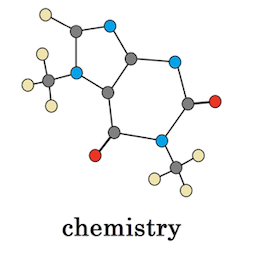
\includegraphics[width=\textwidth]{images/opening page/chemistry.png}    
    \end{minipage}  
    \begin{minipage}{0.31\columnwidth}
    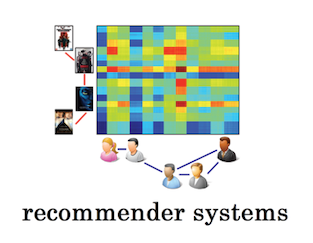
\includegraphics[width=\textwidth]{images/opening page/recommender systems.png}
    \end{minipage}
    \begin{minipage}{0.31\columnwidth}
    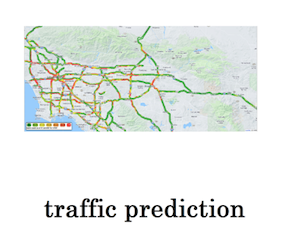
\includegraphics[width=\textwidth]{images/opening page/traffic.png}  
    \end{minipage}
    
    \begin{minipage}{0.3\columnwidth}
    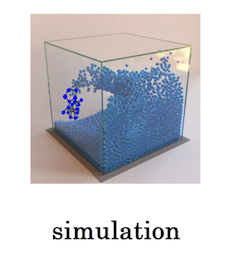
\includegraphics[width=\textwidth]{images/opening page/simulation.png}    
    \end{minipage}  
    \begin{minipage}{0.3\columnwidth}
    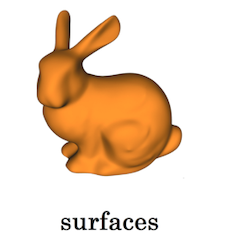
\includegraphics[width=\textwidth]{images/opening page/surfaces.png}
    \end{minipage}
    \begin{minipage}{0.3\columnwidth}
    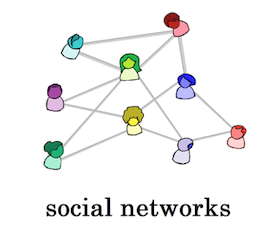
\includegraphics[width=\textwidth]{images/opening page/social networks.png}  
\end{minipage}\hfill  
    
\end{figure}  
    
\end{frame}

\subsection{Notations}

\begin{frame}
\frametitle{Notations}
% START BY INTRODUCING THE NOTATIONS:
% A GRAPH IS AN ORDERED PAIR OF TWO SETS: A SET OF NODES LABELED 1 TO N AND A SET OF PAIRS OF NODES SIGNIFYING CONNECTIONS BETWEEN THEM.
% .
% .
% .
% A: ELEMENTS CAN BE BINARY 0 AND 1 AND THEY CAN BE IN THE RANGE [0,1] IN WHICH CASE THE GRAPH IS SAID TO BE WEIGHTED
% RANDOM: ADJACENCY MATRICES THAT ARE NOT BINARY WILL REPRESENT EDGE/NON EDGE PROBABILITY
% WE DISCUSS UNDIRECTED GRAPH - IF N M IS AN EDGE THEN ALSO M N

\begin{itemize}[itemsep=1em, label=\textbullet]
    \item A \textbf{graph} is a pair $G = ([N], E)$. 
    \item $E\subseteq [N] \times [N]$ is the set of \textbf{edges}.%\pause
    \item A pair $(n,m)\in [N]\times[N]$ is called a \textbf{dyad}.
    % MENTION UNDIRECTED, WEIGHTED
    \item \textbf{Sparse graphs}: $O(|E|) \lll N^2$
    \item An edge between nodes $n$ and $m$ is denoted by $n\sim m$. A non-edge by $n\not\sim m$.%\pause
    \item $\mathbf{A}= \{a_{nm}\in \{0,1\}\}_{n,m = 1}^N$ is the \textbf{adjacency matrix}.%\pause
    \item \textbf{Random Graph Model}: An $N\times N$ matrix with elements $p_{nm} = P(n\sim m)$
    % TO SAY: WEIGHTED + UNDIRECTED
    \item \textbf{Undirected}: $n \sim m \iff m\sim n$
\end{itemize}
\end{frame}

\begin{frame}
\frametitle{Notations}
% ZACHARY: A GRAPH OF FRIENDSHIP CONNECTIONS IN A KARATE CLASS. ON THE LEFT: ADJACENCY 
\begin{figure}
    \begin{minipage}{0.4\columnwidth}
    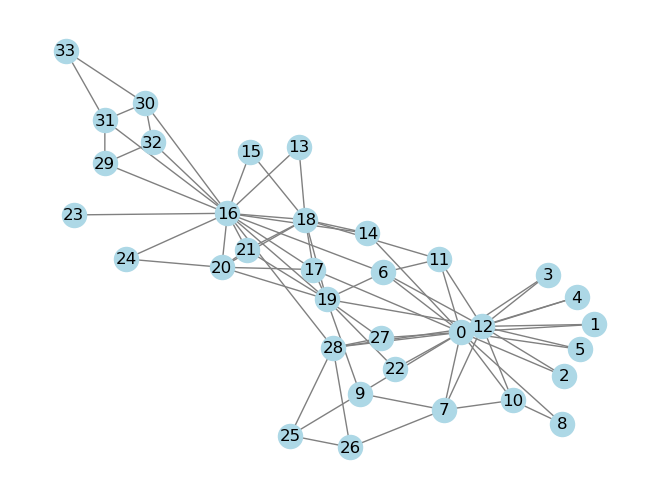
\includegraphics[width=\textwidth]{images/karate_graph.png}    
    \end{minipage}  
    \begin{minipage}{0.3\columnwidth}
    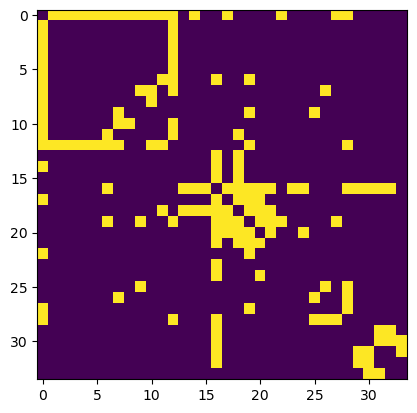
\includegraphics[width=\textwidth]{images/karate_adj.png}       
\end{minipage}\hfill  
    \caption{Zachari's karate club graph and it's adjacency matrix.}
\end{figure}    
\note{aids booger poop}
\end{frame}



\subsection{Graph Representation Learning}
% ---------------------------------------
\begin{frame}{Graph Representation Learning}
    % MAIN TASK OF ML ON GRAPHS.
    % LEARN FEATURES (VECTORS IN R^C) IN OUR CASE FOR EACH NODE (NOT NECESSARILY)  TO CAPTURE THE STRUCTURAL INFORMATIONS
    % FEATURES ARE NOT GIVEN
    % FEATURES ARE USED FOR DOWNSTREAM TASKS
\begin{itemize}[itemsep=1em, label=\textbullet]
    \item Learn a vector $\mathbf{f}_n\in \mathbb{R}^C$ for every node, $C\lll N$.%\pause
    
    $\mathbf{F}\in \mathbb{R}^{N\times C}$ is the matrix whose rows are the features.
    \item The representation captures the \textbf{structural} information. %\pause
    \item Representation is used for downstream tasks:
     
    \textbf{Examples}: Community Detection, Node/Graph Classification, Anomaly Detection, Link Prediction, etc.%\pause
    %TERMINOLOGY: EMBEDDING, REPRESENTATION, EMBEDDING SPACE, CODE SPACE, REPRESENTATION SPACE, LATENT SPACE.
\end{itemize}
    % THE PROBLEM IS HOW TO LEARN THE EMBEDDING SO THAT IS CAPTURES THE STRUCTURE


\begin{figure}
    \begin{minipage}{0.35\columnwidth}
    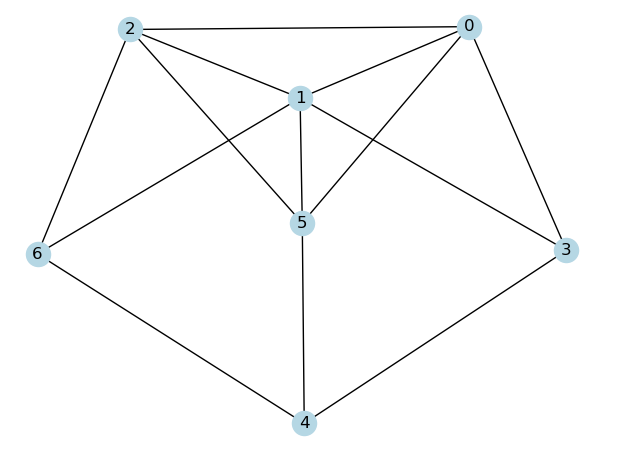
\includegraphics[width=\textwidth]{images/stam_graph.png}    
    \end{minipage}\hspace{0.08\columnwidth}  
    \raisebox{0.5\height}{\makebox[0.05\columnwidth][c]{\Huge$\rightarrow$}}\hspace{0.08\columnwidth}
    \begin{minipage}{0.27\columnwidth}
    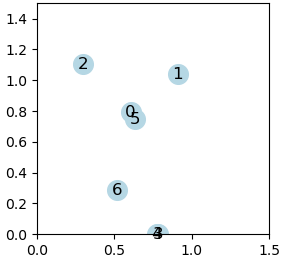
\includegraphics[width=\textwidth]{images/stam_embedding.png}       
    \end{minipage}
\end{figure}

    \centering
    \huge\textcolor{brown}{How to learn the embedding?}

\end{frame}


% -----------------------------------------
\subsection{Autoencoders}
% ----------------------------
% ONE OF THE MOST IMMEDIATE WAYS OF THINKING ABOUT LEARNING THE EMBEDDING IS TO AUTO ENCODE THE GRAPH.
% INTUITIVELY IF THE GRAPH CAN BE RECONSTRUCTED FROM THE EMBEDDING, THE EMBEDDING CAPTURES THE INFORMATION IN THE GRAPH. IF THE STRUCTURE IS ALL THAT IS GIVEN, THEN THE STRUCTURE IS ALL OF THE INFORMATION.
% THE ENCODER GIVES EVERY NODE AN EMBEDDING VECTOR
% THE DECODER TAKES A PAIR OF NODES AND RETURNS A PROBABILITY OF CONNECTING.
% WE OPTIMIZE BY RECONSTRUCTING THE ADJACENCY. IN OUR CASE WE DO THIS BY MAXIMIZING THE LOG PROBABILITY OF RECONSTRUCTING A     
\begin{frame}
\frametitle{Autoencoders}
\begin{itemize}[itemsep=1em, label=\textbullet]
    % immediate way for learning
    \item \textbf{Intuition}: A reconstructable representation captures the structural information.%\pause
    \item \textbf{Encoder} $\mathbf{f}:[N] \rightarrow \mathbb{R}^{N\times C}$ 
    \item \textbf{Decoder} $w: \mathbb{R}^C \times \mathbb{R}^C  \rightarrow [0,1]$. $w(\mathbf{f}_n, \mathbf{f}_m) = P(n\sim m)$ %\pause
    \item Optimize by making $w(\mathbf{f}_n, \mathbf{f}_m)$ similar to $\mathbf{A}$.
    \

\end{itemize}

    \begin{figure}
        \centering
        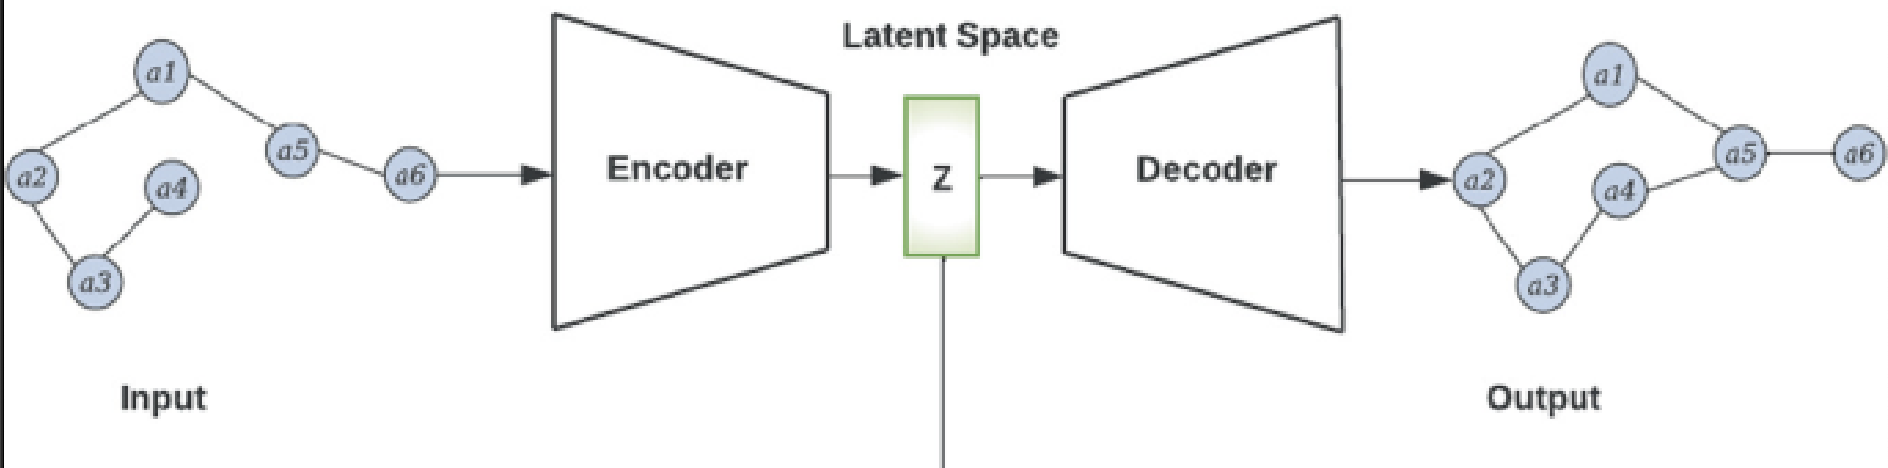
\includegraphics[width=0.9\linewidth]{images/graph_auto.png}
    \end{figure}
\end{frame}
% ---------------------------

\subsubsection{Factorization and Inner Product Decoders}
\begin{frame}
\frametitle{Autoencoders: Factorization and Inner Product Decoders}
% WE WILL DISCUSS A SPECIFIC CLASS OF AUTOENCODERS.
% FACTORIZATION MODEL THE DECODER AS A FUNCTION OF SOME MATRIX PRODUCT OF THE FEATURES OF THE ENCODED NODES, PERHAPS WITH SOME OTHER MATRICES (CAN ALSO BE LEARNED OR CONSTANT).

% INNER PRODUCT METHODS MODEL THE DECODING AS DEPENDENT ON THE INNER PRODUCT BETWEEN FEATURE VECTORS

% BIGCLAM MODELS THE DECODER AS 1- THE EXPONENT OF MINUS THE INNER PRODUCT

% PROXIMITY BASED RECONSTRUCTION OPERATES ON THE SAME LOGIC AND ALSO DEPENDS ON THE INNER PRODUCT (EXPAND THE l2 DISTANCE THROUGH ABBREVIATED MULTIPLICATION FORMULAS)

\begin{itemize}[itemsep=1em, label=\textbullet]
    \item  \textbf{Factorization} based decoders: $w(\mathbf{f}_n, \mathbf{f}_m) = g(\mathbf{f}_n^\top \mathbf{B} \mathbf{f}_m)\approx a_{nm}$.
    % EXPLAIN a_nm is the nm element
    \item \textbf{Inner product} methods assume $w(\mathbf{f}_n, \mathbf{f}_m) = g(\mathbf{f}_n^\top \mathbf{f}_m) \approx a_{nm}$.%\pause
    \item Example: \textbf{BigClam} is an inner product method in which $w(\mathbf{f}_n, \mathbf{f}_m) = 1-e^{-\mathbf{f}_n^\top \mathbf{f}_m} \approx a_{nm}$%\pause
    \item Similarly, proximity based reconstruction learns $w(\| \mathbf{f}_n - \mathbf{f}_m\|_2)\approx a_{nm}$ (Laplacian eigenmaps).%\pause
\end{itemize}




\end{frame}


\begin{frame}{Message Passing}
    \begin{itemize}
        \item Message passing on graphs updates the representation of nodes with aggregated data from neighbors.
    
    \item $\mathbf{m}^{t}_n = \underset{k\in \mathcal{N}(n)}{Aggr}{M^t(\mathbf{f}^t_n,\mathbf{f}^t_k)}$
    \item $\mathbf{f}^{t+1}_n = U^t(\mathbf{m}^t_n, \mathbf{f}^t_n)$
    \vspace{0.3cm}
    \item $R^t = \underset{n\in [N]}{Bggr}(\mathbf{F}^t)$
    \item $Aggr$ and $Bggr$ are permutation invariant (aggregation functions).
    \end{itemize}
\end{frame}
% ---------------

% --------------
\section{Main Contributions}

\begin{frame}
\frametitle{Main Contributions}


% OUR MAIN CONTRIBUTIONS ARE TO INTRODUCE IECLAM AND IT'S EXTENSION PIECLAM WHICH ARE NOVEL FACTORIZATION AUTOENCODER METHODS.

% IECLAM IS BASED OFF OF BIGCLAM WHICH IS A PROVEN EFFECTIVE AND EFFICIENT INNER PRODUCT METHOD

% WE DEFINE A DISTANCE MEASURE BETWEEN EDGE PROBABILITY MATRICES CALLED THE LOG CUT METRIC

% WE PROVE UNIVERSALITY STATEMENTS ABOUT IECLAM THAT FOR A DESIRED PRECISION IN LOG CUT DISTANCE, THE ORDER OF MAGNITUDE OF THE DIMENSION OF THE EMBEDDING SPACE DEPENDS ONLY ON THE PRECISION

% WE SHOW THAT INNER PRODUCT METHODS LIKE BIGCLAM ARE NOT UNIVERSAL, AND THE EMBEDDING DIMENSION OF A GRAPH OF N NODES DEPENDS ON N.

% WE EXTEND THE EMBEDDING SPACE TO A PROBABILITY SPACE TO DEFINE PIECLAM (FROM IECLAM) AND PCLAM (FROM BIGCLAM) THAT ARE GENERATIVE GRAPH MODELS FROM WHICH WE CAN SAMPLE NEW GRAPHS.
\begin{itemize}[itemsep=1em, label=\textbullet]
    \item \textbf{IeClam \& PieClam}: novel factorization autoencoder methods.
    \item IeClam is based off of BigClam which is an effective and efficient inner product autoencoder model.
    \item We define a distance measure between probabilistic graph models called \textbf{log cut} distance, and a concept of \textbf{universality} for graph autoencoders.
    \item \textbf{Universality Theorem} for IeClam, a desired precision $\epsilon$ requires $C(\epsilon)= O(\epsilon^{-2})$ embedding dimension for any graph.%\pause
    \item Previous methods similar to BigClam \textbf{not universal}. %\pause
    \item Extend the embedding space to a probability space - PieClam and PClam are \textbf{generative} versions of IeClam and BigClam.%\pause
    
\end{itemize}
\end{frame}

\section{BigClam Model}

\subsection{Community Affiliation}
\begin{frame}{BigClam: Community Affiliation}
% WE WILL START BY EXPLAINING THE BIGCLAM WHICH IS THE MODEL ON WHICH WE BASE ALL OF THE OTHER MODELS.

% EVEN BEFORE BIGCLAM WE SHOULD EXPLAIN ABOUT WHAT COMMUNITY AFFILIATION IS.
% A COMMUNITY IS A GROUP OF NODES WITH THE SAME STRUCTURAL BEHAVIOR.

% THE NOTION OF A COMMUNITY IS THE SAME AS AUTOENCODED FEATURE EMBEDDINGS BECAUSE COMMUNITIES ARE FEATURES, AND THE GRAPH CAN BE RECONSTRUCTED USING THEM.

% CAN BE BINARY - every node can either belong/not belong, CONTINUOUS - every node is assigned a number that is the strength of belonging, 
% OVERLAPPING - belong to multiple communities, NON OVERLAPPING - a node can't belong to multiple communities

% WE WILL BE DEALING ONLY WITH CONTINUOUS NON OVERLAPPING COMMUNITIES

% INCLUSIVE COMMUNITIES ARE COMMUNITIES IN WHICH STRONG AFFILIATION INCREASES CONNECTION PROBABILITY. 
%IN ADDITION, THE MORE OVERLAPPING COMMUNITIES TWO NODES SHARE THE MORE IT IS LIKELY FOR THEM TO CONNECT. 
% INTUITIVELY THIS IS TRUE ABOUT SOCIAL CONNECTIONS SINCE THE MORE INTERESTS PEOPLE HAVE IN COMMON, EVEN THE MORE FRIENDS THEY HAVE IN COMMON, THE MORE IT IS LIKELY FOR THEM TO CONNECT

% INNER PRODUCT DECODING CAN ONLY EMBED INCLUSIVE COMMUNITIES

    \begin{itemize}[itemsep=1em, label=\textbullet]
    \item \textbf{Community}: a group of nodes with the same structural behavior.
    \item \textbf{Overlapping Communities}: same as autoencoded feature embeddings.
    \item \textbf{Inclusive communities}: common membership increases connection probability.%\pause
    \item \large\textcolor{brown}{Inner product decoding can \textit{only} embed inclusive communities.}
    % EXAMPLE: FRIENDSHIPS FORMING FROM COMMON INTERESTS
    
    \end{itemize}
    \begin{figure}
        \centering
        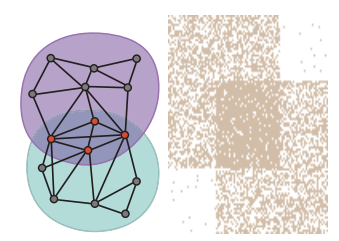
\includegraphics[width=0.3\linewidth]{images/dense_overlap.png}
    \end{figure}
        \centering

\end{frame}



\subsection{Overview}
\begin{frame}
\frametitle{BigClam: Overview}
\begin{itemize}[itemsep=0.7em, label=\textbullet]
    \item \textbf{BigClam Overview:}%\pause
    \begin{itemize}[itemsep=1em, label=\textbullet]
        \item Inner product based (inclusive) overlapping community affiliation model.
        \item $f_n^c \in [0,\infty)$ represents the affiliation of node $n$ to community $c$.
        \item Proven very efficient and effective.%\pause
    \end{itemize}
    
\end{itemize}

\end{frame}

\subsection{Probabilistic Model}
\begin{frame}
\frametitle{BigClam: Probabilistic Model}
\begin{itemize}[itemsep=1em, label=\textbullet]
        % THE BIGCLAM IS DEFINED BY A PROBABILISTIC MODEL CALLED THE POISSON MODEL. WE WILL NOT GO OVER THE POISSON INTERPRETATION, WE CAN JUST SEE THAT THE PROBABILITY OF CONNECTION INCREASES THE MORE FEATURES ARE ALIGNED (HAVE A STRONG INNER PRODUCT).
        % THE PROBABILITY OF DISCONNECTION DECREASES EXPONENTIALLY WITH THE INNER PRODUCT, THE PROBABILITY OF CONNECTION IS THE COMPLEMENT OF THE PROBABILITY FOR DISCONNECTION.
        
        %%%%%%%%%%%%%%  POISSON MODEL %%%%%%%%%%%%%%%%%%%%%
        
        % EXPLAIN WHAT A POISSON MODEL IS
        % the bigclam probabilistic model assumes that the network and all of it's individual pairs are probabilistic,
        % imagine that every pair is actually sampled independently multiple times. the actual pair that appears in the data is a snapshot of these samplings.
        % the GT graph that is generated by this is a collection of realizations one for every pair independently
        % for every node pair, the probability of finding 0 edges (i.e not having an edge between them) is given by poisson distribution (things happen randomly and independently and we are asking about the probability of sampling a number of events, in this case 0, in the snapshot we take)
        % IF YOU WEREN'T FOLLOWING THE EXPLANATION IT'S FINE, REMEMBER THAT A HIGH INNER PRODUCT BETWEEN FEATURES = HIGH CONNECTTIVITY PROBABILITY.

        %%%%%% POISSON EXPLANATION %%%%%%%%%%%%

        % THE PROBABILITY OF THE ENTIRE GRAPH GIVEN THE NODE FEATURES (READ THE FORMULA)
        
        %%% CONDITIONAL PROBABILITY %%%
        % THE RECONSTRUCTION PROBABILITY IS ALWAYS CONDITIONED ON THE FEATURES, AND THE FEATURES ARE OPTIMIZED ACCORDING TO IT.
        \item Non edges are Poisson distributed with mean
        $\mathbf{f}_n^\top \mathbf{f}_m$ ($k=0$). 
         \[P(n \not \sim m | \mathbf{f}_n, \mathbf{f}_m) = e^{-\mathbf{f}_n^\top \mathbf{f}_m}\]%\pause
         \item Therefore
         % COMPLEMENTARY
         \[P(n\sim m| \mathbf{f}_n, \mathbf{f}_m) = 1 - e^{-\mathbf{f}_n^\top \mathbf{f}_m}\]%\pause

         \item The probability for the entire graph is
         % PAIRS ARE INDEPENDENT
         \[ P(E|\mathbf{F}) = \sqrt{\prod_{n \in [N]}\prod_{m \in \mathcal{N}(n)}P( n\sim m|\mathbf{\mathbf{f}_n, \mathbf{f}_m})\prod_{m \notin \mathcal{N}(n)} P( n\not\sim m)|\mathbf{f}_n, \mathbf{f}_m)}\]%\pause
         % READ THE FORMULA OUT LOUD
\end{itemize}

    
\end{frame}


\begin{frame}
\frametitle{BigClam: Loss}
\begin{itemize}[itemsep=1em, label=\textbullet]
        \item The log likelihood is 
    \[ l(\mathbf{F}) = \frac{1}{2}\sumgraph \Big(\sumneighbors{}{\log(1-e^{-\mathbf{f}_n^{\top } \mathbf{f}_m})} - 
 \sumstrangers{\mathbf{f}_n^{\top } \mathbf{f}_m}\Big).\]%\pause
 
\item Optimize by gradient ascent:
    \begin{align}
    \label{eqn:vanilla_optimization}
    \mathbf{F}^{(i+1)} = \mathbf{F}^{(i)} + \delta\nabla_{\mathbf{F}}l({\mathbf{F}}^{(i)}),
    \end{align}%\pause
for some learning rate $\delta>0$.    
\end{itemize}

\end{frame}



\begin{frame}
\frametitle{BigClam: Reparametrization Trick}
\begin{itemize}[itemsep=1em, label=\textbullet]
 % NOTICE THAT THE NON NEIGHBOR TERM HAS A LOT MORE ELEMENTS FOR SPARSE GRAPHS WHICH RESULTS IN A LARGE NUMBER OF OPERATIONS. 
 
 % SO THE BIGCLAM UTILIZES A REPARAMETRIZATION TRICK OF THE SUM TO REPLACE THE NON NEIGHBORS TERM WITH A SUM ON ALL THE NODES TO BE CALCULATED ONCE. THE ONLY TERM THAT CHANGES BETWEEN NODES IS THE SUMMATION ON NEIGHBORS, SO THE NUMBER OF OPERATIONS IS NOW O(E). EVERY NODE IS UPDATED BY AN AGGREGATION OF IT'S NEIGHBORHOOD (MESSAE PASSING) 
\item Reparametrization trick \[2l(\mathbf{F})=
   \sumgraphu \Big(\sumneighbors{\log(e^{\mathbf{f}_n^{\top } \mathbf{f}_n} - 1)}  - \mathbf{f}_n^\top {\sumgraph{\mathbf{f}_m}} + \|\mathbf{f}_n\|^2\Big).\]%\pause
\item The gradient  
\[ \nabla_{\mathbf{f}_n}l = 
    \sumneighbors{\mathbf{f}_m \big(1-e^{-\mathbf{f}_n^\top  \mathbf{f}_m}
    \big)^{-1}} - \sumgraph{\mathbf{f}_m} + \mathbf{f}_n .\]%\pause
    
\end{itemize}
The number of operations is now $O(|E|)$, every node is updated by the same aggregation of it's neighborhood (\textbf{message passing}).
% BLA BLA BIGCLAM GOOOD BLA HAS PROBLAMS

\end{frame}

\begin{frame}{BigClam as Message Passing}
    The feature optimization is implemented as a message passing algorithm.

\begin{equation}
\label{eqn:message passing bigclam}
\begin{aligned}
    &M^t(\mathbf{f}^t_n, \mathbf{f}^t_m) = \mathbf{f}^t_m\left(1-e^{-{\mathbf{f}^t_n}^\top \mathbf{L} \mathbf{f}^t_m}\right)^{-1} \\[1em]
    & \mathbf{m}^{t}_n = \underset{k\in \mathcal{N}(n)}{\sum}{M^t(\mathbf{f}^t_n,\mathbf{f}^t_k)} \\[1em]
    &R^t = \sumgraph \mathbf{f}^t_n \\[1em]
    &\mathbf{f}_n^{t+1} = U(\mathbf{m}^t_n, \mathbf{f}^t_n, \delta) = \mathbf{f}^t_n + \delta(\mathbf{m}^t_n - R^t + \mathbf{f}^t_n) \\
\end{aligned}
\end{equation}

\end{frame}

\section{IeClam}
\subsection{Bipartite Is Not Inclusive}
\begin{frame}{IeClam: Bipartite is not Inclusive}
\hypertarget{bipartite_blindspot}{}
    % AFTER THE SHORT INTRODUCTION WE GET TO THE FIRST PART OF OUR CONTRIBUTION WHICH IS THE IECLAM MODEL
    
    % TO ILLUSTRATE THE MAIN PROBLEM WITH INCLUSIVE COMMUNITY MODELS LET US LOOK AT AN EXAMPLE
    
    % A BIPARTITE GRAPH IS A GRAPH IN WHICH THERE ARE TWO GROUPS CALLED PARTS AND EVERY GROUP IS DISTINGUISHED BY IT'S CONNECTION TO THE OTHER GROUP. THIS CAN BE GENERALIZED IN MANY WAYS TO LARGER STRUCTURES.
    
    % BIPARTITE (OR HETEROPHILIC STRUCTURES) APPEAR IN THE REAL WORLD WHEN YOU COMPETE WITH THE MEMBERS OF YOUR COMMUNITY.
    % WHAT IF m AND n APPLY FOR THE SAME RECRUITER K?
    % DATING (opposites attract), SHOPPING LISTS, JOB SEEKING, A neural network, circuitry...

    % THE BIPARTITE STRUCTURE IS STRICTLY NOT INCLUSIVE BECAUSE OF THE TRIANGLE INEQUALITY LIKE PROPERTY OF THE INNERPRODUCT (EXPLAIN THE TRIANGLE INEQUALITY PROBLEM)

    % IN THE EXAMPLE WE SHOW THE RESULT OF TRAINING BIGCLAM ON A BIPARTITE - THE GREEN NODES TRY TO ALIGN WITH THE ORANGE NODES AND THEY END UP ALIGNING WITH EACH OTHER, CREATING A UNIFORM CONNECTION PROBABILITY - A UNIPART
    % THIS IS ALSO SEEN WHEN THE BIPARTITE IS A PART OF A LARGER GRAPH.
    
    % WE GENERALIZE THE DEFINITION OF COMMUNITY TO ENCOMPASS THIS PROPERTY. 
    
    \begin{figure}
        \begin{minipage}{0.25\columnwidth}
        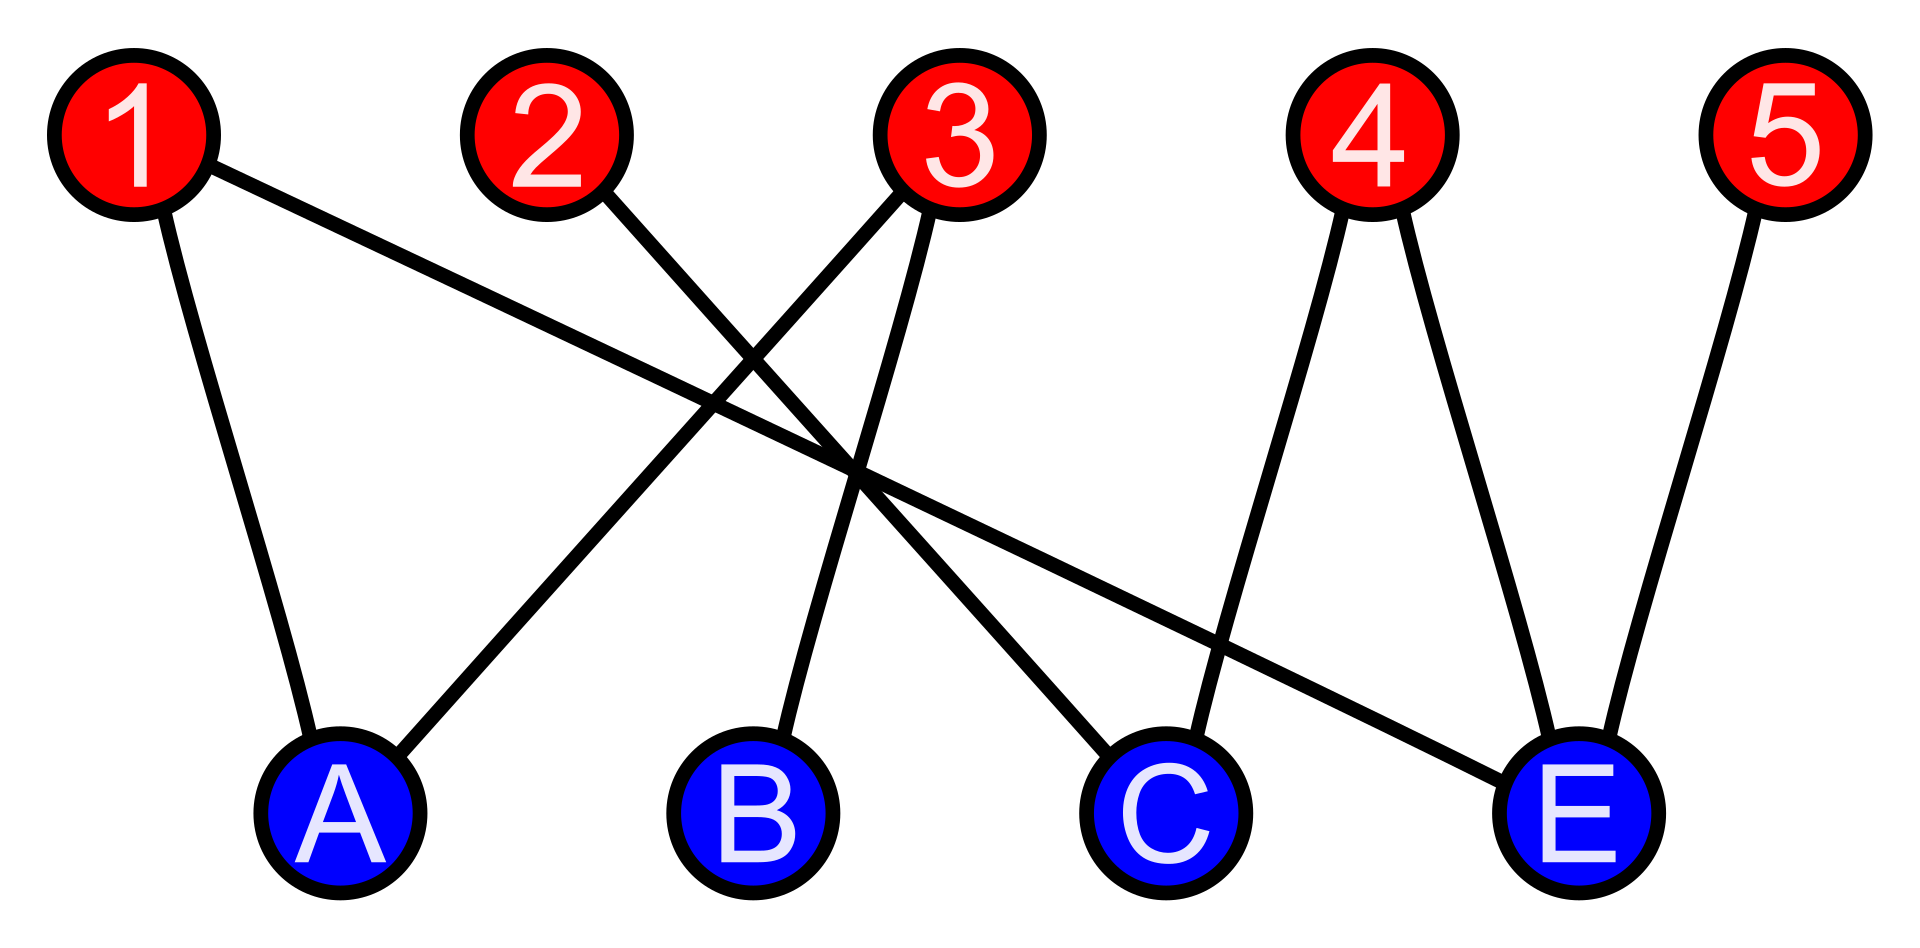
\includegraphics[width=\textwidth]{images/bipart/Simple_bipartite_graph;_two_layers.png}    
        \end{minipage} \hspace{3em} 
        \begin{minipage}{0.25\columnwidth}
            
\includegraphics[width=\textwidth]{images/bipart/bipart_gt.png}
        \end{minipage}
        
    \end{figure}
    \textbf{Triangle inequality}: if $n\sim k$ and $m\sim k$ then $\mathbf{f}_{n}^\top \mathbf{f}_k$ and $\mathbf{f}_{m}^\top \mathbf{f}_k$ are large and therefore $\mathbf{f}_n^\top \mathbf{f}_m$ is also large which implies $m\sim n$ with high probability.%\pause
    \begin{figure}    
        \begin{minipage}{0.25\columnwidth}
            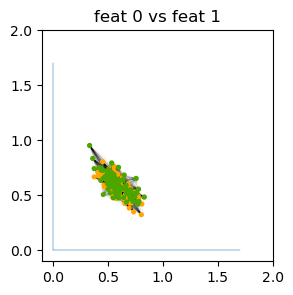
\includegraphics[width=\textwidth]{images/bipart/feat_bipart_big.png}
        \end{minipage}
        \hspace{3em}
        \begin{minipage}{0.25\columnwidth}
        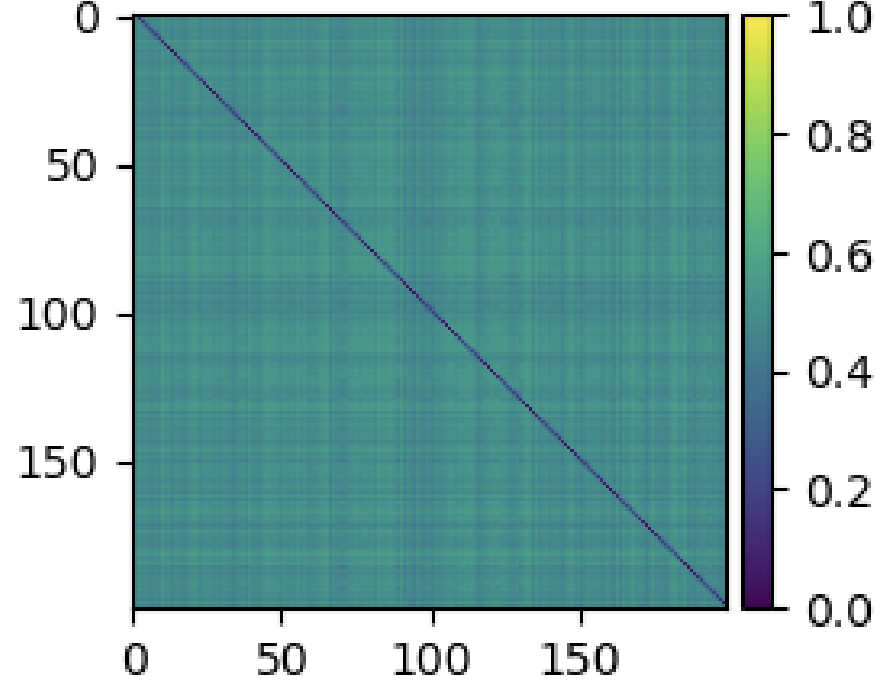
\includegraphics[width=\textwidth]{images/bipart/bipart_decode_bigclam.png}       
        \end{minipage}\hfill
        \caption{Bipartite autoencoding with BigClam}
    \end{figure}
        
\end{frame}

\begin{frame}{IeClam: Bipartite is not Inclusive}
Inclusive model decodes bipartite as one inclusive community.

        % SHOW THIS ONLY IF WE ARE LESS THAN 20 MINS!!!!!!!
        % BIGCLAM TURNS HETEROPHILIC PARTS INTO UNIPARTS ALSO FOR LARGER STRUCTURES:
        % IN HERE WE SEE A GRAPH COMPOSED OF TWO PARTS, ONE OF WHICH IS BIPARTITE. THE BIGCLAM FINDS THE TWO PARTS, BUT THE BIPARTITE PART IS ENCODED INTO AN INCLUSIVE COMMUNITY 
\begin{figure}     
        \begin{minipage}{0.25\columnwidth}
            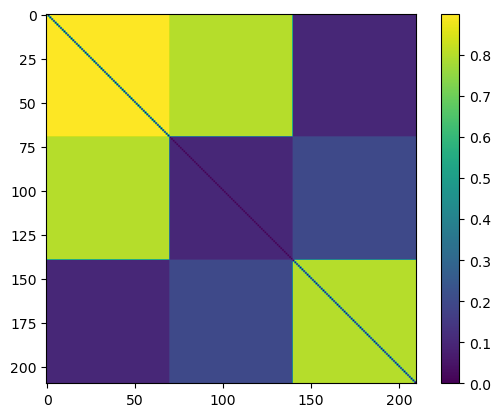
\includegraphics[width=\textwidth]{images/bipart/tripart/tripart.png}
        \end{minipage}
        \begin{minipage}{0.25\columnwidth}
        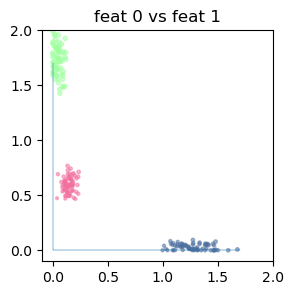
\includegraphics[width=\textwidth]{images/bipart/tripart/feats_bigclam_tripart.png}       
        \end{minipage}
        \begin{minipage}{0.25\columnwidth}
        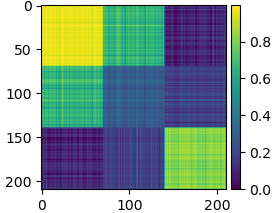
\includegraphics[width=\textwidth]{images/bipart/tripart/tripart_bigclam_decode.png}       
        \end{minipage}
    \end{figure}
    
\end{frame}

\subsection{Exclusive Communities}
% THIS ECENTIVISES US TO DEFINE A NEW TYPE OF COMMUNITY
%  WE GENERALIZE THE DEFINITION OF COMMUNITY TO ENCOMPASS THE EXCLUSIVITY PROPERTY. 
\begin{frame}{IeClam: Exclusive Communities}
    \begin{itemize}[itemsep=1em, label=\textbullet]
        \item \textbf{Exclusive community}: a community for which common membership \textit{reduces} the probability to connect. 
        \item Two nodes with a high score for the same exclusive community $c$ should have a lower connection probability for it.
        \item Denote inclusive communities with $\mathbf{t} \in \mathbb{R}^C$ and exclusive communities with $\mathbf{s}\in\mathbb{R}^C$.%\pause
    \end{itemize}
\end{frame}

\subsection{Probabilistic Model}
\begin{frame}{IeClam: Probabilistic Model}
    \begin{itemize}[itemsep=1em, label=\textbullet]   
    \item The representation for node $n$ will be: $\mathbf{f}_n = (\mathbf{t}_n, \mathbf{s}_n)$.%\pause
    
    % THE ORDER OF THE INCLUSIVE AND EXCLUSIVE COMMUNITIES DOESN'T MATTER, BUT WE CONCATENATE THEM ONE AFTER THE OTHER.
    \item Instead of inner product use \textbf{L-Product}: \[\mathbf{f}_n^\top \mathbf{L} \mathbf{f}_m = \mathbf{t}_n^\top \mathbf{t}_m - \mathbf{s}_n^\top \mathbf{s}_m\]
    % COMMON MEMBERSHIP IN INCLUSIVE RAISES CONNECTION PROB, COMMON MEMBERSHIP IN EXCLUSIVE COMMUNITY REDUCES CONNECTION PROB.
    % FOR THE MODEL TO REMAIN PROBABILISTIC, t*t > s*s
    \item The single edge probability is now:
    %INSTEAD OF INNER PROD
    \[P(n \sim m| \mathbf{f}_n, \mathbf{f}_m) = 1-e^{-\mathbf{f}_n^\top \mathbf{L} \mathbf{f}_m}\] 
    Where $\mathbf{L} = {\rm diag}(1,\dots, 1, -1, \dots, -1)$ 
    % \[2=\mathbf{f}_n^\top \mathbf{f}_m}\]%\pause
    \item \textbf{Notice}: for a probabilistic model $\mathbf{f}_n^\top \mathbf{L} \mathbf{f}_m \geq 0 \iff \mathbf{t}_n^\top \mathbf{t}_m \geq \mathbf{s}_n^\top \mathbf{s}_m$ .
    \end{itemize}
        
    \end{frame}

\begin{frame}{IeClam: Probabilistic Model}
    \begin{itemize}[itemsep=1em, label=\textbullet]   
    \item \textcolor{brown}{Inner product has been replaced by $L$ product.}
    \item The log likelihood
    \[ l(\mathbf{F}) = \frac{1}{2}\sumgraph \Big(\sumneighbors{}{\log(1-e^{-\mathbf{f}_n^\top \mathbf{L} \mathbf{f}_m})} - 
 \sumstrangers{\mathbf{f}_n^\top \mathbf{L} \mathbf{f}_m}\Big).\]%\pause
 
\item Reparametrization trick \[2l(\mathbf{F})=
   \sumgraphu \Big(\sumneighbors{\log(e^{\mathbf{f}_n^\top  \mathbf{L} \mathbf{f}_n} - 1)}  - \mathbf{f}_n^\top \mathbf{L} {\sumgraph{\mathbf{f}_m}} + \mathbf{f}_n^\top \mathbf{L} \mathbf{f}_n \Big).\]%\pause
\item The gradient  
\[ \nabla_{\mathbf{f}_n}l = 
    \mathbf{L}\bigg(\sumneighbors{\mathbf{f}_m \big(1-e^{-\mathbf{f}_n^\top \mathbf{L} \mathbf{f}_m}
    \big)^{-1}} - \sumgraph{\mathbf{f}_m} + \mathbf{f}_n \bigg).\]%\pause
\item Complexity stays $O(|E|)$.
    \end{itemize}
        
    \end{frame}

\subsection{Bipartite Encoding}
    % FOR A GROUP OF NODES TO BE EXCLUSIVE AND STAY A PROBABILISTIC MODEL IT NEEDS TO ALSO HAVE AN INCLUSIVE PART TO GET CANCELED WITH THE EXCLUSIVE PART
    \begin{frame}{IeClam: Bipartite Encoding}
        \begin{itemize}[itemsep=1em, label=\textbullet]
            \item A bipartite graph $\mathbf{A}$ can be encoded by embedding part 1 to $(b,b)$ and part 2 to $(b,-b)$ where $b\in \mathbb{R}_+$. 
            \[w(\mathbf{f}_n, \mathbf{f}_m) = 
            \begin{cases} 
                1-e^{-b^2} & \text{if $m, n$ \textbf{not} the same part} \\
                0 & \text{otherwise}
            \end{cases}
        \]
            \item $w(\mathbf{f}_n, \mathbf{f}_m) \to \mathbf{A} \quad \text{as} \quad b \to \infty$.%\pause
    \end{itemize}
    % USING AN EXCLUSIVE COMMUNITY WE CAN APPROXIMATE A BIPARTITE
    % a AND -a ARE THE MOST EXTREME VALUES FOR EXCLUSIVE COMMUNITIES FOR THE MODEL TO STAY PROBABILISTIC (IN 2D, THE RESTRICTION ON THE SPACE BECOMES A RESTRICTION ON COMMUNITY VALUES), 
    \begin{figure}
        \begin{minipage}{0.2\columnwidth}
        
\includegraphics[width=\textwidth]{images/bipart/bipart_gt.png}    
        \end{minipage}  
        \begin{minipage}{0.4\columnwidth}
            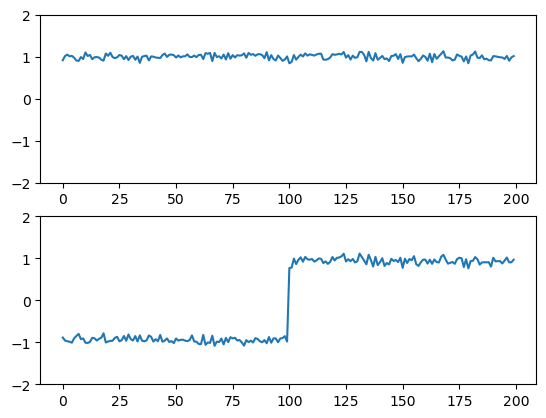
\includegraphics[width=\textwidth]{images/bipart/feats_bipart_ie.png}
        \end{minipage}
        \begin{minipage}{0.2\columnwidth}
        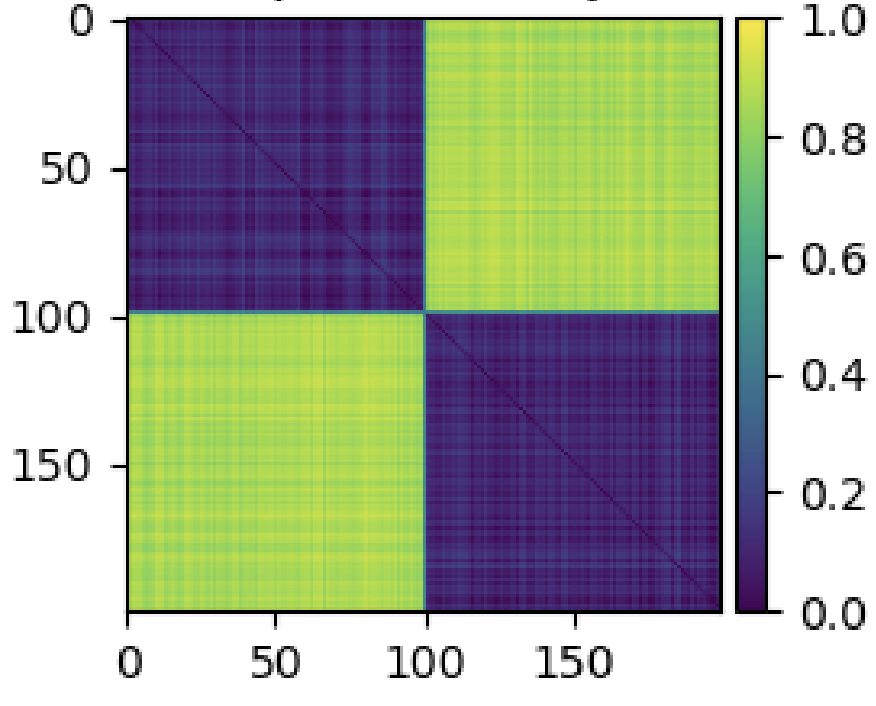
\includegraphics[width=\textwidth]{images/bipart/bipart_decode_ieclam.png}       
        \end{minipage}\hfill  
       
    \end{figure}

    \end{frame}
    
\subsection{L and Positivity Domain}
% WONT GO OVER THE WHOLE RESTRICTION PROCESS, ONLY THAT WE SET THE SAME NUMBER OF INCLUSIVE AND EXCLUSIVE AND PAIR THEM UP, CREATING A SENSE OF GENERALIZED COMMUNITIES AND KEEPING EVERYTHING POSITIVE

\begin{frame}{IeClam: $\mathbf{L}$ and Positivity Cones}
\begin{itemize}[itemsep=1em, label=\textbullet]
    \item The bilinear form $\mathbf{L}$ is \textbf{not} an inner product.%\pause
    % GOOD: NO TRIANGLE INEQUALITY. BAD: NOT POSITIVE.
    \item \textbf{Positive probabilities}: restrict the community affiliation space to $\mathcal{C} \subset  \mathbb{R}^{2C}$ s.t $\forall \mathbf{f}, \mathbf{g}: \mathbf{f}^\top \mathbf{L} \mathbf{g}>0 .$%\pause
    \item For simplicity, we further restrict $\mathbb{R}^{2C}$ to pairwise cones \[\mathcal{T} = \{\mathbf{f}=(\mathbf{t}, \mathbf{s}) s.t. \forall c\in[C]: |s^c| \leq t^c\}\]
    \item $\implies$ The most exclusive you can get is on $s^c=\pm t^c$.
    % CONE RESTRICTION: THE SAME WAY THAT IT WAS CONVENIENT FOR 2D, IT'S ALSO CONVENIENT TO DO FOR MULTIPLE DIMENSIONS, ALSO, T,S PAIRS ARE NOW INTERPRETABLE AS GENERALIZED COMMUNITIES BECAUSE OF THE CONES AND BECAUSE OF THE NEXT SLIDE:
\end{itemize}
\end{frame}
\begin{frame}{IeClam: Pairwise Cones - Intuition}
    \begin{itemize}[itemsep=1em, label=\textbullet]
    \item We can think of $(s^c,t^c)$ as one complex feature $f^c = t^c + is^c = r^ce^{i\theta^c}$.
    \item For two nodes: ${\mathbf{f}_1^c}^\top \mathbf{L} \mathbf{f}_2^c = \mathcal{R}(f_1^c f_2^c) = r_1r_2\cos(\theta_1 + \theta_2)$   
    \begin{figure}
        \centering
        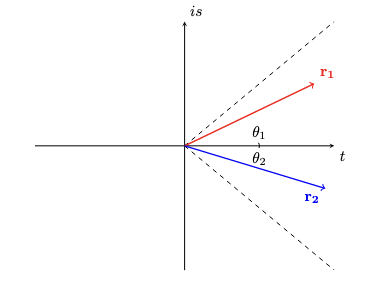
\includegraphics[width=0.5\linewidth]{images/cones/cone_intuition.png}
    \end{figure}
    \item $\implies$ The most exclusive you can get is on $s=\pm t$.
    \end{itemize}
\end{frame}


\begin{frame}{Pairwise Cones: Examples}
        \begin{figure}
        \begin{minipage}{0.2\columnwidth}
        
\includegraphics[width=\textwidth]{images/bipart/bipart_gt.png}    
        \end{minipage}  
        \begin{minipage}{0.19\columnwidth}
            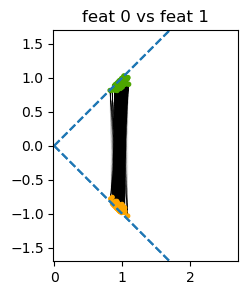
\includegraphics[width=\textwidth]{images/bipart/timecone_bipart_ie.png}
        \end{minipage}
        \begin{minipage}{0.2\columnwidth}
        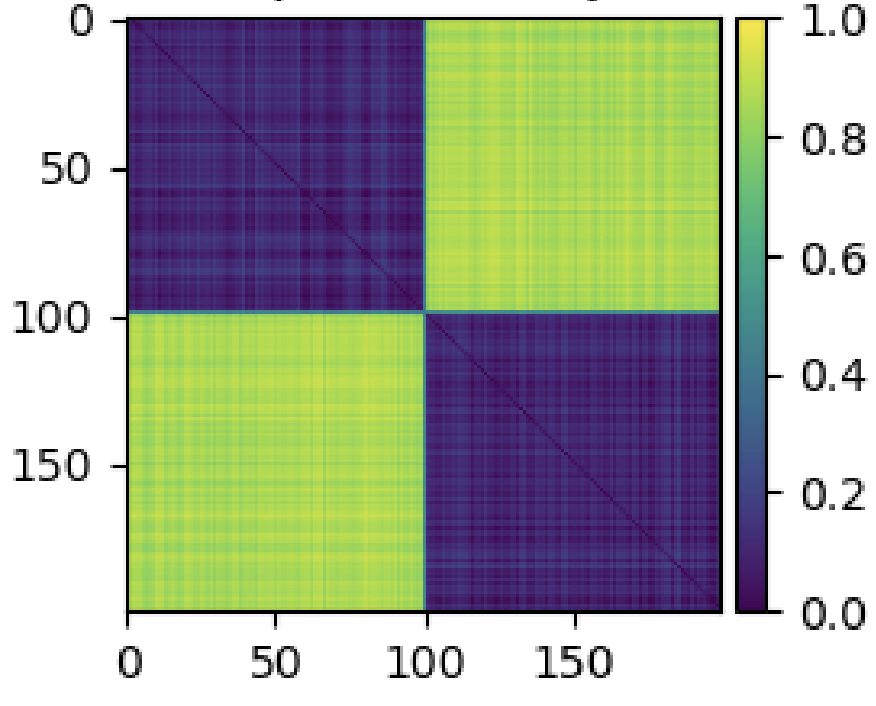
\includegraphics[width=\textwidth]{images/bipart/bipart_decode_ieclam.png}       
        \end{minipage}\hfill  
        \end{figure}
    \rule{\textwidth}{0.4pt}
            \begin{figure}
        \begin{minipage}{0.2\columnwidth}
        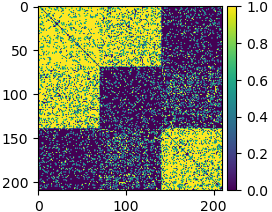
\includegraphics[width=\textwidth]{images/bipart/tripart/gt.png}    
        \end{minipage}  
        \begin{minipage}{0.19\columnwidth}
            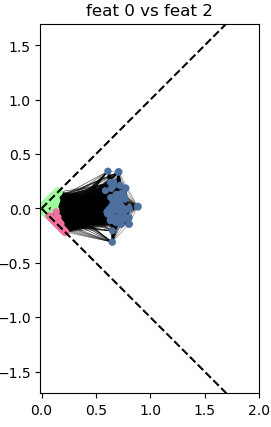
\includegraphics[width=\textwidth]{images/bipart/tripart/inclusive.png}
        \end{minipage}
        \begin{minipage}{0.2\columnwidth}
        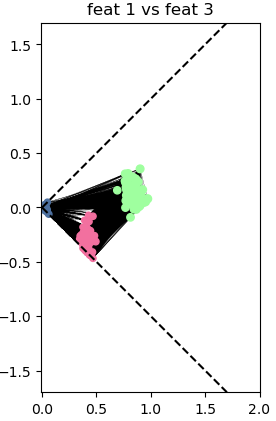
\includegraphics[width=\textwidth]{images/bipart/tripart/inclusive_exclusive.png}       
        \end{minipage}
        \begin{minipage}{0.2\columnwidth}
        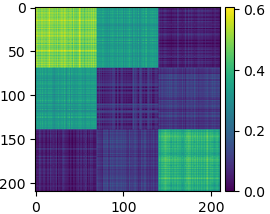
\includegraphics[width=\textwidth]{images/bipart/tripart/decoded.png}       
        \end{minipage}
        \end{figure}

        

\end{frame}

\section{PieClam}

\subsubsection{Generative Models}
\begin{frame}
\frametitle{PieClam: Generative Models}
% IN ADDITION, ANOTHER MODIFICATION WE MADE IS TO MAKE THE AUTOENCODING GENERATIVE
%BEFORE TALKING ABOUT PIECLAM WE SHOULD GIVE SOME BACKGROUND ON GENERATIVE MODELS.
% HAVE NO CONTEXT
\begin{itemize}[itemsep=1em, label=\textbullet]
    \item $P(E | \mathbf{F})$ restricted to the training graph.
    % IECLAM AND BIGCLAM LEARN A CONDITIONAL PROBABILITY IN THAT THERE IS NO SENSE OF THE PROBABILITY OF THE REPRESENTATION FEATURES THEMSELVES
    % TO GENERALIZE MUST LEARN JOINT DISTRIBUTION
    \item Learn the joint probability distribution $P(E \wedge \mathbf{F})$.%\pause
    \item \textbf{Motivation}: 
    \\1. Generate new graphs by sampling. %\pause
    % WE WOULD HAVE LIKED TO LEARN FROM THE TRAINING DATA HOW TO GENERATE NEW GRAPHS
    \\2. Infer the likelihood of other graphs.%\pause
\end{itemize}
\end{frame}

\subsubsection{Prior on Code Space}
\begin{frame}
\frametitle{PieClam: Prior on Code Space}
\begin{itemize}[itemsep=1em, label=\textbullet]
%PIECLAM IS IECLAM WITH PRIOR ON THE CODE SPACE, PCLAM IS BIGCLAM WITH PRIOR ON THE CODE SPACE
    \item Define a prior probability density function code space.%\pause
    \item Using Bayes' law: \[p(E\wedge \mathbf{F}) = P(E|\mathbf{F})p(\mathbf{F})\]%\pause
    \item Assume independence of feature events: \[p(\mathbf{F}) = \prod_{n\in[N]}p(\mathbf{f}_n)\]%\pause

    \item The probabilistic model will now be: \[ p(E\wedge \mathbf{F}) = \underbrace{\prod_{n \in [N]}p(\mathbf{f}_n)}_{p(\mathbf{F})}\underbrace{\bigg(\sqrt{\prod_{m \in \mathcal{N}(n)}P( n\sim m|\mathbf{F})\prod_{m \notin \mathcal{N}(n)} P( n\not\sim m|\mathbf{F}})\bigg)}_{P(E|\mathbf{F})}\]%\pause
    % NOTICE THAT THE MODEL NOW IS A PROBABILITY DENSITY FUNCTION AND NOT ACTUAL PROBABILITY!
    % THE JOINT PROBABILITY IS THE PRODUCT OF ALL OF THE EDGES MULTIPLIED BY THE PRODUCT OF ALL OF THE NODES,
        
\end{itemize}
\end{frame}


\subsubsection{Probabilistic Model and PClam}

\begin{frame}{PieClam: Probabilistic Model and PClam}
    \begin{itemize}[itemsep=1em, label=\textbullet]
        \item log likelihood loss:
        \[l(\mathbf{F})=
   \sumgraphu \Bigg(\frac{1}{2}\Big(\sumneighbors{\log(e^{\mathbf{f}_n^\top  \mathbf{L} \mathbf{f}_n} - 1)}  - \mathbf{f}_n^\top \mathbf{L} {\sumgraph{\mathbf{f}_m}} + \mathbf{f}_n^\top \mathbf{L} \mathbf{f}_n \Big) + \log\big(p(\mathbf{f}_n)\big)\Bigg).\]%\pause
   \item The prior acts as \textbf{regularization} - attractive force.%\pause
   % THE LOSS IS A SUM OF INTERACTION FORCES FROM NEIGHBORS AND NON NEIGHBORS, AND AN EXTERNAL "POTENTIAL" FIELD.
   % THE PRIOR MAKES ALL NODES ATTRACT ONE ANOTHER.
   \item \textbf{PClam}: BigCalm with prior.%\pause 
    \item Model the prior as a \textbf{neural network} $p(\mathbf{f}|\alpha)$.  
    \end{itemize}
\end{frame}


\subsubsection{Normalizing Flows Neural Network Prior}
\begin{frame}{PieClam: Normalizing Flows Neural Network Prior}
    \begin{itemize}[itemsep=1em, label=\textbullet]
        \item An invertible transformation $\mathbf{z}$ from the affiliation probability space to a gaussian probability space. %\pause
        % ALLOWS SAMPLING!
        % COMPOSITION OF TRANSFORMATIONS
        \item  The transformation is scaled so the distribution stays normalized.%\pause
        \[p(\mathbf{f}) = G\Big(\mathbf{z}(\mathbf{f})\cdot|\det(\partial_f{\mathbf{z}})|\Big)\]
        %NEURAL NETWORK EXPRESSIVE.%\pause
        %SAMPLING IN THE OTHER DIRECTION.%\pause
        \item Maximize log likelihood of the features.
    \end{itemize}
    \begin{figure}
        \centering
        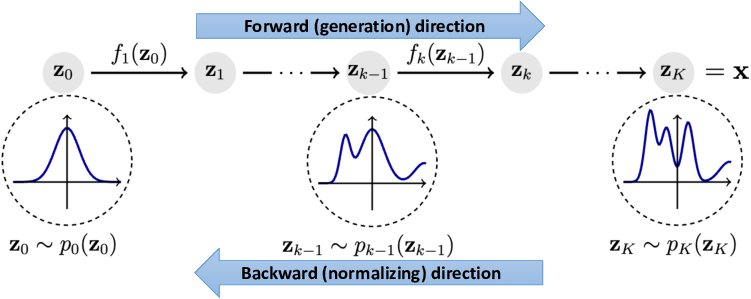
\includegraphics[width=0.8\linewidth]{images/normflow.png}
    \end{figure}
\end{frame}

\subsubsection{Optimizing PieClam}
\begin{frame}{PieClam: Optimizing PieClam}
%MOVE TO THE BOTTOM
    \begin{itemize}[itemsep=1em, label=\textbullet]
        \item \textbf{Node initialization}: random positions according to gaussian in the middle of $\mathbb{R_+^C}$ or $\mathcal{T}$.
        \item Run \textbf{alternating} optimization on the affiliation features $\mathbf{f}$ and prior parameters $\alpha$.
        \item Optimize each of the two losses with \textbf{gradient ascent}.
        % WHEN FEATURES OPTIMIZE THE PRIOR IS CONSTANT, WHEN PRIOR OPTIMIZES FEATURES ARE CONSTANT.
        \item \textbf{Feature regularization}: $l_1$ regularization.
        \item \textbf{s regularization}: $l_1$ regularization on the $\mathbf{s}$ communities.
        \item \textbf{Prior regularization}: Noise addition and weight decay.
        % ADD NOISE TO THE FEATURES WHEN TRAINING THE PRIOR TO PREVENT THE PRIOR FROM COLLAPSING AROUND NODES.
        \item \textbf{More hypers}: learning rate and number of iterations for feats and prior optimizations, number of alternations, learning rate scheduler.
    \end{itemize}
\end{frame}

\subsubsection{PieClam as Graphon}
\begin{frame}{PieClam as Graphon}
    
\begin{itemize}[label=\textbullet]
\item A graph generative model that extends SBMs.
\item Can be seen as a weighted graph with a ``continuous'' node set $[0,1]$. 
\end{itemize}

\begin{definition}
The space of graphons $\mathcal{W}$ is defined to be the set of all measurable functions  $W:[0,1]^2\rightarrow [0,1]$ which are symmetric, namely $W(x,y)=W(y,x)$. 
\end{definition}
\begin{itemize}[label=\textbullet]
\item The edge weight $W(x,y)$ of a graphon $W\in \mathcal{W}$ can be seen as the probability of having an edge between node $x$ and node $y$.
\item A random graph is generated by sampling  independent uniform nodes $\{X_n\}$ from the graphon domain $[0,1]$, and connecting each pair $X_n,X_m$ in probability $W(X_n,X_m)$.
\end{itemize}
\end{frame}


\begin{frame}{PieClam as Graphon}
    
% Note that the prior $p$ defines a standard atomless probability space over the community affiliation space $\mathbb{R}^K$. 
% Since all standard atomeless probability spaces are equivalent,
\begin{itemize}[label=\textbullet]
    \item There is a probability preserving a.e. bijection  $\xi_p:[0,1]\rightarrow\mathbb{R}^K$ that maps the prior probability to the uniform probability over $[0,1]$ (another NF layer). 
    \item Sample $N$ points $\{X_n\}_{n=1}^N\subset[0,1]$ uniformly. Observe that $\{\xi_p(X_n)\}_{n=1}^N\subset \mathbb{R}^K$ are indepndent samples via the probability density $p$.
    \item Connect the points according to the BigClam or IeClam models $P(n\sim m| \xi_p(X_n),\xi_p(X_m))$.

This shows that PClam and PieClam coincide with the generative graphon model. 
\end{itemize}
\end{frame}


\subsubsection{Sampling Graphs}
% FEATURES AND PRIOR ARE OPTIMIZED TOGETHER UNTILL THE PROCESS CONVERGES
\begin{frame}{PieClam: Sampling Graphs}
Sample a graph with $N$ nodes from PClam or PieClam,
    \begin{itemize}[itemsep=1em, label=\textbullet]
        \item Sample affiliation vectors $(\mathbf{f}_n)_{n=0}^N\sim p(\cdot)$. 
        \item Connect the nodes with probability $P(n\sim m|\mathbf{f}_n, \mathbf{f}_m) = 1 - e^{\mathbf{f}_n^\top L \mathbf{f}_m}$.%\pause
    \end{itemize}
    \begin{figure}
        \centering
        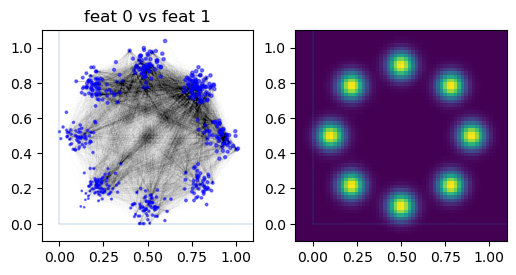
\includegraphics[width=0.5\linewidth]{images/sample circle.png}
    \end{figure}
    
\end{frame}

\subsubsection{Graphs With Node Features}
\begin{frame}{PieClam: Graphs With Node Features}
    \begin{itemize}[itemsep=1em, label=\textbullet]
        \item Definition: a \textbf{graph-signal} is the ordered triplet $([N], E, \mathbf{X})$, $\mathbf{X} \in \mathbb{R}^d$ are \textbf{node features} given with the data.%\pause
        % THE NODE FEATURES X COME WITH THE GRAPH AND ARE NOT DIRECTLY RELATED TO THE STRUCTURE, BUT THE TWO CAN BE CONNECTED (PROBABLY USUALLY ARE)
        \item Examples: user info, protein composition, social media groups etc.%\pause
        \item PieClam (and Pclam) for a graph-signal: concatenate $(\mathbf{f}_n, \mathbf{x}_n)$ when learning the prior.%\pause
    \end{itemize}    
\end{frame}




\section{Universality of PieClam}

\subsection{Universal Autoencoders}

\begin{frame}
\frametitle{Universal Autoencoders}
For some distance measure for $d(\cdot, \cdot)$
\begin{definition}[Universal Autoencoder]    
    A family of code spaces $\mathbb{R}^M$ and corresponding pairwaise decoders $D_M:\mathbb{R}^{2M}\rightarrow[0,1]$, parametrized by $M\in\mathbb{N}$, is called  \emph{universal} if for every $\epsilon>0$ there is $M\in\mathbb{N}$ (which depends only on $\epsilon$) such that for every $N\in\mathbb{N}$ and every graph  with adjacency matrix $\mathbf{A}$ and $N$ nodes there are $N$ points in the code space $\{z_n\in\mathbb{R}^M\}_{n=1}^N$ such that 
     \[d(\mathbf{D}_M(\mathbf{z}), \mathbf{A}) <\epsilon.\] 
\end{definition}
\end{frame}



\subsection{Cut Distance}
\begin{frame}{Universality: Cut Distance}
\begin{itemize}[itemsep=1em, label=\textbullet]
% UNIVERSALITY MEANS THAT FOR A GIVEN PRECISION, THERE IS AN EMBEDDING IN A DIMENSIONAL SPACE WHOSE DIMENSION DOES NOT DEPEND ON THE NUMBER OF NODES IN THE GRAPH. 

    %%% INTRODUCTION %%%%%
    % TO PROVE UNIVERSALITY WE SHOULD FIRST DEFINE THE DISTANCE METRICS THAT WE WILL BE USING. WE NEED A DISTANCE METRIC POR DIFFERENCE BETWEEN PROBABILISTIC GRAPH MODELS - PROBABILISTIC MATRICES LIKE THE ONES WE HAVE BEEN DISCUSSING.

    %%% CUT NORM %%%%
    % WE WILL BUILD OUR DISTANCE METRIC FROM AN EXISTING DISTANCE METRIC BETWEEN GRAPHS CALLED THE CUT METRIC. THE ADVANTAGE OF THIS METRIC IS THAT IT LOOKS AT THE EDGE DENSITY PROPERTY OF A GRAPH, WHICH IS WHY IT'S USED IN APPROXIMATION THEOREMS FOR GRAPHS AND RANDOM GRAPH MODELS.

    % WE WILL FIRST DEFINE THE CUT NORM WHICH INDUCES THE CUT METRIC.
    % THE CUT NORM MEASURES NORM OF A GRAPH BY THE TWO SETS OF NODES BETWEEN WHICH THERE IS THE DENSEST CONNECTIVITY. IN OTHER WORDS THE SIZE OF THE LARGEST CUT - THE TWO SETS OF NODES IN THE GRAPH THAT CUTTING THEM WILL REMOVE THE MOST EDGES.
    
    %%% CUT METRIC %%%%%
    % THE CUT NORM DEFINES A CUT METRIC, WHICH IS THE CUT NORM OF A DIFFERENCE OF MATRICES.
    % THE CUT METRIC OF A AND B IS THE RECTANGLE UXV (SETS OF NODES) ON WHICH THEIR EDGE ENTRIES ARE THE MOST DIFFERENT.

  \item The \textbf{cut norm} of a matrix $\mathbf{X}\in\mathbb{R}^{N\times N}$ is defined to be:
    \begin{equation}
  \|\mathbf{X}\|_{\square}:=\frac{1}{N^2}\sup_{\mathcal{U},\mathcal{V}\subset[N]}\Big|\sum_{i\in \mathcal{U}}\sum_{j\in \mathcal{V}}x_{i,j}\Big|.
\end{equation}  

\item The \textbf{cut metric} between matrices $\mathbf{A}$ and $\mathbf{B}$ is $\|\mathbf{A}-\mathbf{B} \|_{\square}$ 

%  A AND B HAVE THE SAME NUMBER OF NODES.

\end{itemize}
    
\end{frame}


\subsection{Log Cut Distance}
\begin{frame}{Universality: Log Cut Distance}
    \begin{itemize}[itemsep=1em, label=\textbullet]
    %     \item Define the \textbf{Log Cut Norm} for a random graph model $P=\{ 0 \leq p_{nm} < 1\}$:
    % \[          
    % \|\mathbf{\log(1-P)}\|_{\square}:=\frac{1}{N^2}\sup_{\mathcal{U},\mathcal{V}\subset[N]}\bigg(\Big|\log\Big(\prod_{i\in \mathcal{U}}\prod_{j\in \mathcal{V}}(1-p_{ij})\Big)\Big|\bigg).
    % \]
    % \textbf{Interpretation}: The most unprobable rectangle in the probabilistic graph model.
    \item The \textbf{Log Cut Metric}:
    \[
        D_{\square}(\mathbf{P} || \mathbf{Q}):=  \frac{1}{N^2}\sup_{\mathcal{U},\mathcal{V}\subset[N]}\Bigg(\Big|\log\Big(\prod_{n\in \mathcal{U}}\prod_{m\in \mathcal{V}}
\frac{1-p_{n,m}}{1-q_{n,m}}\Big)\Big|\Bigg)\]
  \[= \|\log(1-\mathbf{P})- \log(1-\mathbf{Q}) \|_{\square}\]
\textbf{Interpretation}: The biggest part of the model $P$ that can't be explained by the model $Q$.
    
    
    \end{itemize}
\end{frame}

\begin{frame}{Universality - Log cut Distance}
\begin{itemize}[itemsep=2em, label=\textbullet]
   \item If one of the matrices has elements 1 (e.g. a \textbf{realization} $\mathbf{A}$), regularization is added and penalized:
\small
$\mathbf{P}$ and $\mathbf{A}$ is defined to be
    \[
    D_{\square}(\mathbf{P} || \mathbf{A}):= 
    \inf_{0< d\leq1} \Bigg( d+ \frac{1}{N^2}\sup_{\mathcal{U},\mathcal{V}\subset[N]}\Big|\log\Big(\prod_{n\in \mathcal{U}}\prod_{m\in \mathcal{V}}
\frac{1-p_{n,m}}{1-(1-d)a_{n,m}}\Big)\Big|\Bigg).
    \]
    \item This version of the log cut is used in the universality theorem.
\end{itemize} 

    
    
    % IN OTHER WORDS, WHEN ONE OF THE MATRICES IS A REALIZATION, A REGULARIZATION D IS ADDED AND PENALIZED.

\end{frame}


% \begin{frame}{Universality: Log Cut Distance}
    
% \begin{itemize}[itemsep=1em, label=\textbullet]
%     \item We define a new graph similarity measure for graphs with random edges.
% % FOR PROBABILISTIC RANDOM GRAPH WE WOULD LIKE A DISTANCE MEASURE THAT WILL REFLECT THE DIFFERENCE IN PROBABILISTIC MODELS, AND CORRESPOND WITH THE CUT METRIC ABOVE.



% \begin{definition}
% Given two random graphs over the nodes set $[N]$, with independently Bernoulli distributed edges, with probabilities $\mathbf{P}=\{0 \leq p_{n,m} < 1\}_{n,m\in[N]}$ and $\mathbf{Q}=\{0\leq q_{n,m} < 1\}_{n,m\in[N]}$ respectively, their \emph{log cut distance} is defined to be 
% \small
% \[
%         D_{\square}(\mathbf{P} || \mathbf{Q}):=  \frac{1}{N^2}\sup_{\mathcal{U},\mathcal{V}\subset[N]}\Bigg(\Big|\log\Big(\prod_{n\in \mathcal{U}}\prod_{m\in \mathcal{V}}
% \frac{1-p_{n,m}}{1-q_{n,m}}\Big)\Big|\Bigg).
% \]
% \end{definition}   
% \end{itemize}
% % BREAK DOWN THE EXPRESSION:
% % LOG OF PRODUCT IS SUM OF LOGS SO IT'S THE CUT DISTANCE BETWEEN THE TWO LOG LIKELIHOOD MODELS OF NON EDGES.
% % IN AN EQUIVALENT MANNER TO HOW THE CUT DISTANCE MEASURES DISCREPENCY BY USING THE BIGGEST RECTANGLE, THE LOG CUT MEASURES THE DIFFERENCE IN PROBABILISTIC MODELS BY FINDING THE LARGEST RECTANGLE ON WHICH THEY ARE DIFFERENT, AND THE LOG TERM TURNS THE EXPRESSION TO A CUT DISTANCE BETWEEN THE MATRICES. 


% \end{frame}

% \begin{frame}{Universality - Log cut Distance}
%    If one of the matrices has elements 1 (e.g. a \textbf{realization}), regularization is added and penalized:
%     \begin{definition}{Log Cut Distance}
% Given an unweighted graph with adjacency matrix $\mathbf{A}\in\{0,1\}^{N\times N}$ and a random graph over the nodes set $[N]$, with independently Bernoulli distributed edges with probabilities $\mathbf{P}=\{0\leq p_{nm}<1\}_{nm\in[N]}$, the log cut distance between 
% \small
% $\mathbf{P}$ and $\mathbf{A}$ is defined to be
%     \[
%     D_{\square}(\mathbf{P} || \mathbf{A}):= 
%     \inf_{0< d\leq1} \Bigg( d+ \frac{1}{N^2}\sup_{\mathcal{U},\mathcal{V}\subset[N]}\Big|\log\Big(\prod_{n\in \mathcal{U}}\prod_{m\in \mathcal{V}}
% \frac{1-p_{n,m}}{1-(1-d)a_{n,m}}\Big)\Big|\Bigg).
%     \]
%     % IN OTHER WORDS, WHEN ONE OF THE MATRICES IS A REALIZATION, A REGULARIZATION D IS ADDED AND PENALIZED.
% \end{definition}

% \end{frame}

\subsection{Universal Autoencoders with Log Cut}

\begin{frame}
\frametitle{Universal Autoencoders with Log Cut}
\begin{definition}[Universal Autoencoder]
    % For universality we want to prove that there is a dimension for which there is an encoding that can be decoded, for every graph independent of the number of nodes
    A family of code spaces $\mathbb{R}^M$ and corresponding pairwaise decoders $D_M:\mathbb{R}^{2M}\rightarrow[0,1]$, parametrized by $M\in\mathbb{N}$, is called  \emph{universal} if for every $\epsilon>0$ there is $M\in\mathbb{N}$ (which depends only on $\epsilon$) such that for every $N\in\mathbb{N}$ and every graph  with adjacency matrix $\mathbf{A}$ and $N$ nodes there are $N$ points in the code space $\{z_n\in\mathbb{R}^M\}_{n=1}^N$ such that 
     \[D_{\square}(\mathbf{D}_M(\mathbf{z}) || \mathbf{A}) <\epsilon.\] 
\end{definition}
\end{frame}
% A FAMILY OF DECODERS: A TYPE OF DECODERS. D_M TAKES TWO VECTORS OF LENGTH M.
% FOR AMY NUMBER OF NODES, THEY CAN BE ENCODED AND DECODED INTO AN AT MOST M DIMENSIONAL SPACE.



\subsection{Universality of IeClam and PieClam}


% We give two versions for the universality result. The first is without a cone restriction, and requires a relatively small number of communities for the given error tolerance. 
%The corresponding decoder produces edge weights that can be negative. 
%The second theorem is restricted to the pairwise cone of non-negativity, and has pessimistic  asymptotics for the required number of communities given an error tolerance. This decoder is guaranteed to produce proper edge probabilities in $[0,1)$.



\begin{frame}{Universality in $\mathbb{R}^{2K}$}
    We prove that IeClam (and consequently PieClam) is universal.
\begin{theorem}
\label{thm:IEUniversality}
    For every epsilon $\epsilon>0$, every $N\in\mathbb{N}$, and every adjacency matrix $\mathbf{A}\in[0,1]^{N\times N}$, there are $N$ affiliation features $\mathbf{F}\in \mathbb{R}^{2K}$ of dimension  $K=-9\frac{\log(\frac{\epsilon}{2})^2}{\epsilon^2}$ such that the corresponding IeClam model $\mathbf{P}=\{P(n\sim m|\mathbf{f}_n, \mathbf{f}_m)\}_{n,m=1}^N$ satisfies 
     \[D_{\square}(\mathbf{P} || \mathbf{A}) <\epsilon.\] 
    As a result, 
    IeClam and PieClam are universal autoencoders with code space $\mathbb{R}^{2K}$.
\end{theorem}

Universality in the unrestricted space requires $O(\epsilon^-2)$ communities.
% VERY GOOD ASYMPTOTICS, THOUGH THIS DOESN'T GUARENTEE POSITIVE PROBABILITIES!
\end{frame}


\subsection{Universality in  $\mathcal{T}$}
\begin{frame}{Universality in $\mathcal{T}$}
    
\begin{theorem}
    For every epsilon $\epsilon>0$, every $N\in\mathbb{N}$, and every adjacency matrix $\mathbf{A}\in[0,1]^{N\times N}$, there are $N$ affiliation features $\mathbf{F}$ in the cone of pairwise non-negativity  $\mathcal{T}\subset \mathbb{R}^{2C}$ of dimension  $C=2^{4\lceil -\log(\epsilon/2)^2/\epsilon^2\rceil}$  such that the corresponding IeClam model $\mathbf{P}=\{P(n\sim m|\mathbf{f}_n, \mathbf{f}_m)\}_{n,m=1}^N$ satisfies 
%      \[D_{\square}(\mathbf{P} || \mathbf{A}) <\epsilon
%      \] 
    IeClam and PieClam are universal autoencoders with code space $\mathcal{T}$.
\end{theorem}
Universality in positivity cones is $O(2^{\frac{1}{\epsilon^2}})$ (unrealistically huge!)
% FOR PRECISION OF 0.1 WE WILL NEED 2^100 COMMUNITIES! (STILL UNIVERSAL)
% POSITIVE PROBABILITIES GUARANTEED
\end{frame}

\subsection{BigClam and PClam Are Not Universal}
\begin{frame}{BigClam and PClam Are Not Universal}

    \begin{itemize}[itemsep=1em, label=\textbullet]
        \item For BigClam and PClam we show that the dimension of the embedding space will have to \textbf{depend on the number of nodes} in the graph.
        \item \hyperlink{bipartite_blindspot}{The proof is similar to what was shown in a previous slide.}
    \end{itemize}
\end{frame}





\section{Experiments and Results}

\begin{frame}
\frametitle{Experiments}
\begin{itemize}[itemsep=1em, label=\textbullet]
    \item \textbf{Experiment Overview:}
    \begin{itemize}[itemsep=1em, label=\textbullet]
        \item Synthetic prior reconstruction.%\pause
        \item Synthetic SBM approximation with distance metrics.%\pause
        \item Anomaly detection.%\pause
    \end{itemize}
    \item \textbf{Key Results:}%\pause
    \begin{itemize}[itemsep=1em, label=\textbullet]
    \item synthetic priors in two dimensions are visibly reconstructed only from the graph structure.%\pause
    \item Off diagonal SBMs are decoded well with Ieclam and PieClam and badly by BigClam and PClam.%\pause  
    \item PieClam and IeClam are competative as an anomaly detectors.%\pause
    \item PieClam is compentative as an anomaly detector on graph-signals without using the node features.%\pause
    \end{itemize}
\end{itemize}
\end{frame}

\subsection{Reconstructing Synthetic Priors}
\subsubsection{Description}
\begin{frame}{Experiments: Synthetic Priors - Description}
    \begin{itemize}[itemsep=1em, label=\textbullet]
        \item Sample nodes from synthetic priors and try to learn the prior.%\pause
        \item Resample the affiliation vectors from a standard gaussian in the middle of the code space.%\pause
        \item We optimize BigClam, PClam, IeClam and PieClam to reconstruct the shape they were sampled from, and learn the prior.%\pause
        
    \end{itemize}
    \begin{figure}
        \begin{minipage}{0.3\columnwidth}
            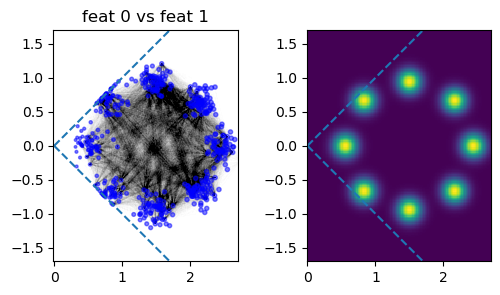
\includegraphics[width=\textwidth]{images/synthetic_2d/circ_ie_gt.png}
        \end{minipage}
        \begin{minipage}{0.3\columnwidth}
        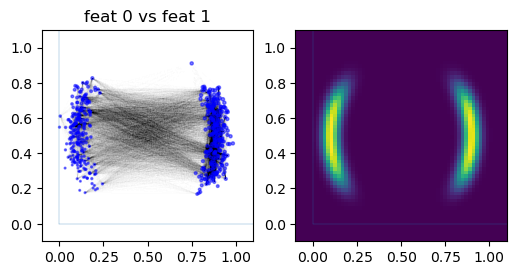
\includegraphics[width=\textwidth]{images/synthetic_2d/moons_big_gt.png}    
        \end{minipage}  
    \end{figure}
\end{frame}

\subsubsection{Results}
\begin{frame}{Experiments: Synthetic Priors - Results}
    \begin{itemize}[itemsep=0.5em, label=\textbullet]
        
    \item Priors have been reconstructed to a similar degree.%\pause
    \item Shape also reconstructed with BigClam and IeClam.%\pause
    \item Prior regularizes results.
    \end{itemize}
    
    \begin{figure}[h]
    \centering
    % Top row with small images
    \begin{minipage}{0.17\textwidth}
        \centering
        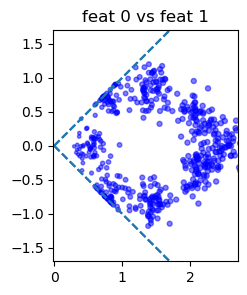
\includegraphics[width=\textwidth]{images/synthetic_2d/circ_ie_reconstruct.png}
    \end{minipage}
    \hspace{0.25\textwidth}
    \begin{minipage}{0.2\textwidth}
        \centering
        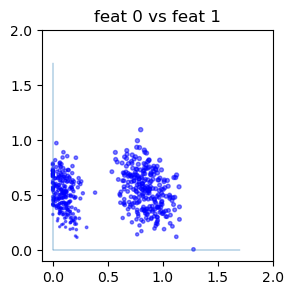
\includegraphics[width=\textwidth]{images/synthetic_2d/moons_big_reconstruct.png}
    \end{minipage}

    % Bottom row with large images
    \vspace{1em} % Add some vertical space between rows
    \begin{minipage}{0.45\textwidth}
        \centering
        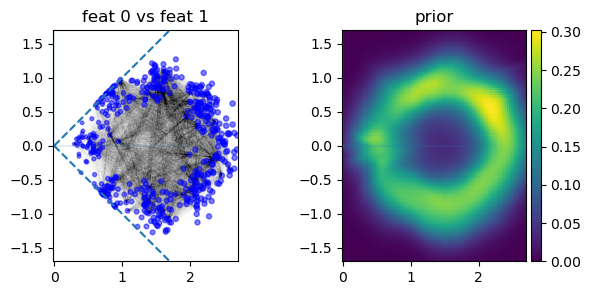
\includegraphics[width=\textwidth]{images/synthetic_2d/piegam_circ_reconstruct.png}
    \end{minipage}
    \vspace{1em} % Add some vertical space between images
    \begin{minipage}{0.45\textwidth}
        \centering
        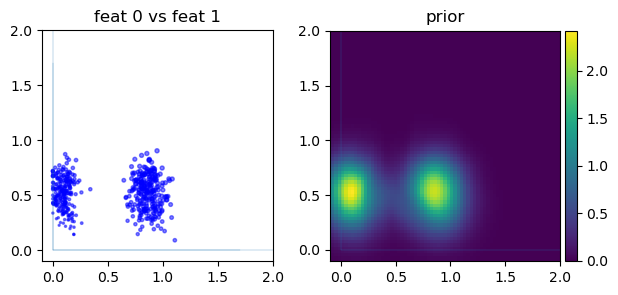
\includegraphics[width=\textwidth]{images/synthetic_2d/moons_pclam_reconstructed.png}
    \end{minipage}
\end{figure}

\end{frame}



\subsection{SBM Distance Measurement}
\subsubsection{Description}
\begin{frame}{Experiments: SBM Distance Measurement - Description}
    \begin{itemize}[itemsep=1em, label=\textbullet]
    \item We sample graphs from the SBMs shown below.%\pause
    \item We approximate the SBMs with the four models and measure the cut, log cut and l2 distances.%\pause 
    \end{itemize}
    \begin{figure}
        \centering
        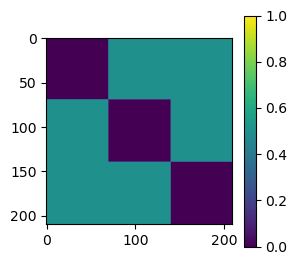
\includegraphics[width=0.3\linewidth]{images/sbm_reconstruction/halfdiag.png}
    \end{figure}
\end{frame}

\subsubsection{Results}
\begin{frame}{Experiments: SBM Distance Measurement - Results}
    \begin{itemize}[itemsep=1em, label=\textbullet]
        
        \item Inclusive methods can't learn exclusive structures.%\pause
        \item Inclusive Exclusive methods reach lower losses.%\pause
        \item Exclusive methods find the SBMs well.
    \end{itemize}
        
        \begin{figure}
            \centering
             \begin{minipage}{0.2\textwidth}
        \centering
        
\includegraphics[width=\textwidth]{images/sbm_reconstruction/halfdiag_ieclam/4_com/adj_cropped.png}
        \end{minipage}
        \begin{minipage}{0.6\textwidth}
        \centering
        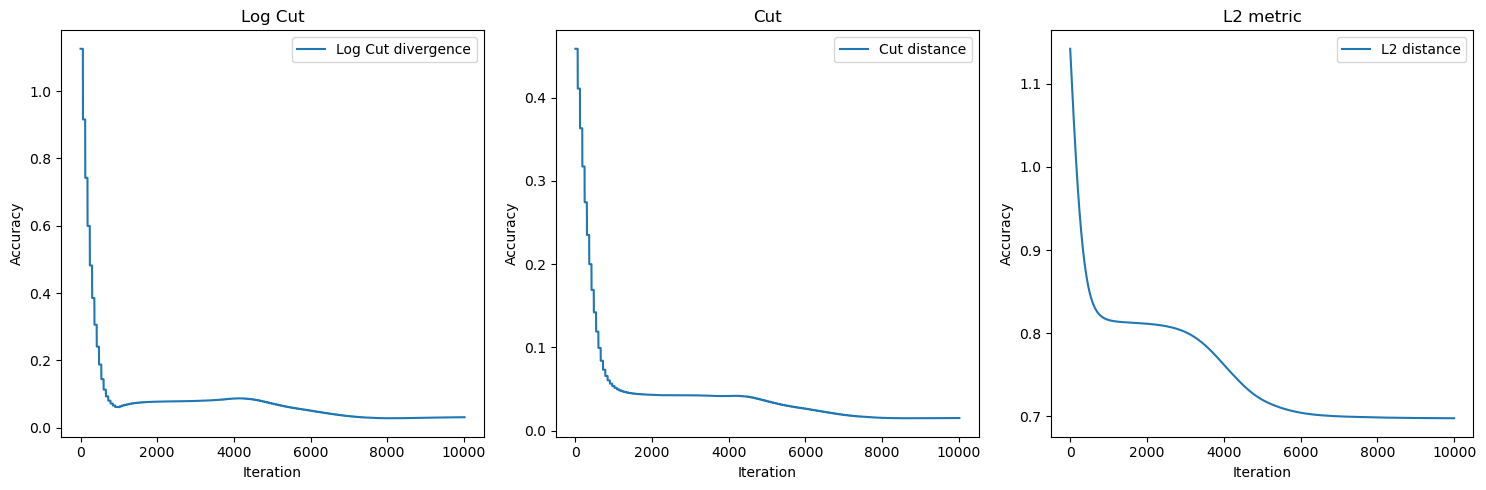
\includegraphics[width=\textwidth]{images/sbm_reconstruction/halfdiag_ieclam/4_com/dists.png}
        \end{minipage}
        \end{figure}


        \begin{figure}
            \centering
             \begin{minipage}{0.2\textwidth}
        \centering
        
\includegraphics[width=\textwidth]{images/sbm_reconstruction/halfdiag_bigclam/4_com/adj_cropped.png}
        \end{minipage}
        \begin{minipage}{0.6\textwidth}
        \centering
        
\includegraphics[width=\textwidth]{images/sbm_reconstruction/halfdiag_bigclam/4_com/distances.png}
        \end{minipage}
        \end{figure}
        
\end{frame}

\subsection{Anomaly Detection}
\subsubsection{Description}
\begin{frame}{Experiments: Anomaly Detection - Description}
\begin{itemize}[itemsep=1em, label=\textbullet]
    \item Calculate node probability and classify with AUC score.
    
    \item Probability calculation:
    \begin{itemize}[itemsep=0.5em, label=\textbullet]
        
        \item star probability \textbf{(S)}
        \item Prior probability \textbf{(P)}
        \item (P) + (S) \textbf{(PS)}
        % THE PROBABILITY FOR THE ENVIRONMENT FOR EVERY NODE
    \end{itemize}
    \item Compare to state of the art, datasets with real anomalies: reddit, elliptic, photo.
\end{itemize}
    
\end{frame}

\subsubsection{Results}
\begin{frame}{Anomaly Detection - Results}
\Large
Using node features.
\begin{table}
\small
\centering
\begin{tabular}{|c|c|c|c|}
    \hline
  Method  & Reddit& Elliptic& Photo\\
    \hline

 (S)- IeClam& \textbf{0.639}& 0.440&\textbf{0.592}\\
 (S) - PieClam& 0.6320 ± 0.0054&  
0.4354 ± 0.0005&*0.5727 ± 0.0151\\
 (P) - PieClam& 0.5089 ± 0.0219& \textbf{0.6201 ± 0.0176}&0.4252 ± 0.0074\\
 (PS) - PieClam& *0.6329 ± 0.0052& \underline{0.5294 ± 0.0089}&0.5289 ± 0.0127\\
 (S) - BigClam & \underline{0.637}& 0.434&\underline{0.581}\\
 \hline
 DOMINANT  & 0.511& 0.296&0.514\\
 AnomalyDAE &0.509& *0.496&0.507\\
 OCGNN  &0.525 & 0.258&0.531\\
 AEGIS &0.535 & 0.455&0.552\\
 GAAN &0.522 &0.259 &0.430\\
 TAM &0.606 & 0.404 & 0.568\\
 \hline
\end{tabular}
\caption{ First place in \textbf{boldface}, second with \underline{underline}, third with *star.}
\end{table}
\end{frame}

\begin{frame}
\Large
Without node features - Still competative!
\begin{table}
\scriptsize
\centering
\begin{tabular}{|c|c|c|c|}
    \hline
  Method  & Reddit & Elliptic & Photo \\
    \hline
  (S) - PieClam & 0.6320 ± 0.0054 & 0.4354 ± 0.0005 & \textbf{0.5727 ± 0.0151} \\
  (P) - PieClam & 0.5089 ± 0.0219 & \textbf{0.6201 ± 0.0176} & 0.4252 ± 0.0074 \\
  (PS) - PieClam & *0.6329 ± 0.0052 & \underline{0.5294 ± 0.0089} & 0.5289 ± 0.0127 \\
    \hline
  (S) - PieClam (No Attr) & \underline{0.6346 ± 0.0015} & 0.4349 ± 0.0009 & *0.5696 ± 0.0065 \\
  (P) - PieClam (No Attr) & 0.4530 ± 0.0142 & *0.4826 ± 0.0134 & 0.4977 ± 0.0747 \\
  (PS) - PieClam (No Attr) & \textbf{0.6351 ± 0.0015} & 0.4349 ± 0.0009 & \underline{0.5697 ± 0.0065} \\
    \hline
\end{tabular}
\caption{Comparison of attributed and unattributed PieClam anomaly detection.}
\label{Table22}
\end{table}
    
\end{frame}

\section{Conclusion}

\begin{frame}
\frametitle{Conclusion}
\begin{itemize}[itemsep=1em, label=\textbullet]
    \item \textbf{Summary:}
    \begin{itemize}[itemsep=1em, label=\textbullet]
        \item IeClam extends BigClam to include both inclusive and exclusive communities.
        \item PieClam and PClam extend IeClam and BigClam to generative models.
        \item Proven universality in autoencoding any graph.
        \item Effective in graph anomaly detection, synthetic reconstruction.
    \end{itemize}
    \item \textbf{Future Work:}
    \begin{itemize}[itemsep=1em, label=\textbullet]
        \item Better Extension of PieClam to incorporate node features in edge probabilities.
        \item Modifications for very sparse datasets.
        \item Link prediction, node classification, etc.

    \end{itemize}
\end{itemize}
\end{frame}

\begin{frame}{Conclusion}
    \Huge
    Questions?
\end{frame}







\section{Proofs}
\begin{frame}{BigClam Is Not Universal}
\begin{itemize}[itemsep=0.5em, label=\textbullet]
 
\item Consider the bipartite graph $\mathbf{B}$ with $N$ nodes at each part, and probability $1-e^{-a^2}$ for an edge between the two parts, and $0$ within each part.  
\item Let $\mathbf{P} = 1-e^{-\mathbf{F}^\top \mathbf{F}}$ be a decoded BigClam graph from the affiliation features $\mathbf{F}$.

\item Denote $\tilde{\mathbf{P}}$ and $\tilde{\mathbf{B}}$ by  
\[\tilde{p}_{n,m}=-\log(1-p_{n,m})=\mathbf{f}_n^\top\mathbf{f}_m,\] 
\[\tilde{b}_{n,m}=-\log(1-b_{n,m})\]
\end{itemize}    
\begin{claim}
    Under the above construction, 
    \[D^0_{\square}(\mathbf{P} || \mathbf{B}) \geq \frac{a^2}{16}.\]
    % As a result, BigClam is not a universal autoencoder.
\end{claim}

\end{frame}

\begin{frame}{BigClam Is Not Universal}

 \textbf{Proof}

Note that $\tilde{b}_{n,m}=a^2$ if $n,m$ are in opposite parts, and $\tilde{b}_{n,m}=0$ if $n,m$ are on the same side.
We index the nodes such that $[N]$ is the first side of the graph, and $[N]+N$ is the second side. For $n\in[N]$ we denote $\mathbf{q}_n=\mathbf{f}_n$ and  $\mathbf{y}_n=\mathbf{f}_{n+N}$.
Next, we use the identity 
\[D^0_{\square}(\mathbf{P} || \mathbf{Q}) = \| \tilde{P}-\tilde{B}\|_{\square },\]
and bound the right-hand-side from below.
\end{frame}

\begin{frame}{BigClam Is Not Universal}
    
First, by the definition of cut norm, for every $\mathcal{U},\mathcal{V}\subset[2N]$,
\[\| \tilde{P}-\tilde{B}\|_{\square} \geq \Big|\frac{1}{4N^2}\sum_{n\in \mathcal{U}}\sum_{m\in \mathcal{V}} (\tilde{p}_{n,m} - \tilde{b}_{n,m})\Big|.\]
Hence, for $\mathcal{U}_1=\mathcal{V}_1=[N]$, $\mathcal{U}_2=\mathcal{V}_2=[N]+N$, $\mathcal{U}_3=[N],\mathcal{V}_3=[N]+N$, and $\mathcal{U}_4=[N]+N,\mathcal{V}_4=[N]$, we have
\[\| \tilde{P}-\tilde{B}\|_{\square} \geq \]
\[\frac{1}{16N^2}\sum_{j=1}^4 \Big|\sum_{n\in \mathcal{U}_j}\sum_{n\in \mathcal{V}_j} (\tilde{p}_{n,m} - \tilde{b}_{n,m})\Big| \]
\[= \frac{1}{16N^2}\sum_{n=1}^N\sum_{m=1}^{N} \mathbf{q}_n^\top \mathbf{q}_m  + \frac{1}{16N^2}\sum_{n=1}^N\sum_{m=1}^{N} \mathbf{y}_n^\top \mathbf{y}_m \]
\begin{equation}
    \label{eq:ClamNpUni0}
    +\frac{1}{8N^2}\sum_{n=1}^N\sum_{m=1}^{N} ( a^2 -\mathbf{q}_n^\top \mathbf{y}_m).
\end{equation}
\end{frame}

\begin{frame}{BigClam Is Not Universal}
    
Denote 
\[\mathbf{q}=\frac{1}{N}\sum_{n=1}^N \mathbf{q}_n, \quad \mathbf{y}=\frac{1}{N}\sum_{n=1}^N \mathbf{y}_n.\]
With these notations, (\ref{eq:ClamNpUni0}) can be written as
\[\| \tilde{P}-\tilde{B}\|_{\square} \geq \]
\[\frac{1}{16}\bigg(\mathbf{q}^\top \mathbf{q}  + \mathbf{y}^\top \mathbf{y} +2\Big|a^2 -\mathbf{q}^\top \mathbf{y}\Big|\bigg) = \]
\begin{equation*}
\begin{cases}
    
\frac{1}{16}\Big(a^2 + (\mathbf{q}^\top-\mathbf{y}^\top)(\mathbf{q}-\mathbf{y})\Big) \geq \frac{a^2}{16} & \text{if} \quad a^2 > \mathbf{q}^\top \mathbf{y} \\
\frac{1}{16}\Big(a^2 + (\mathbf{q}^\top-\mathbf{y}^\top)(\mathbf{q}-\mathbf{y})\Big) \geq \frac{a^2}{8} & \text{otherwise} 
\end{cases}
\end{equation*}

In either case, the claim is proven. 
\begin{flushright}
$\Box$
\end{flushright}
\end{frame}

\begin{frame}{BigClam With No Self Loops Approximating Bipartite Graphs}

If we redefine the BigClam decoder to have no self-loops, namely, $\mathbf{P}$ has entries 
$p_{n,m}=P(n\sim m|\mathbf{f}_n, \mathbf{f}_m)$ for $n\neq m$, and $p_{n,m}=0$ for $n=m$, then one can obtain a bipartite $\mathbf{P}$ with $C=N^2$ communities as follows. 
    
Encode each node $n\in[N]$ in part 1 to $\mathbf{f}_n$ with
$f_n^c=a$ for $c\in (n-1)N + [N]$ and $f_n^c=0$ otherwise. Encode every node $n\in [N]+N$ from side 2 to $\mathbf{f}_n$ with
$f_n^c=a$ for $c\in ([N]-1)N+n$ and $f_n^c=0$ otherwise. It is easy to see that the corresponding $\mathbf{P}$ is bipartite with edge probability between the parts being $1-e^{-a^2}$.
\end{frame}






\begin{frame}{PieClam Is Universal}
    
The proof is based on a version of the weak regularity lemma for intersecting communities. 

% While the standard weak regularity lemma \cite{weakReg,Szemeredi_analyst} partitions the graph into disjoint communities, it is well known that allowing the communities to overlap allows using much less communities, which improves the asymptotics of the approximation.
\begin{definition}
    A (hard) intersecting community graph (ICG) with $N$ nodes and  $K$ communities is a matrix $\mathbf{C}\in\mathbb{R}^{N\times N}$ of the following form. There exist $K$ column vectors $\mathbf{Q}=\big(\mathbf{q}_k\in\{0,1\}^N\big))_{k=1}^K\in \{0,1\}^{N\times K}$ and $k$ coefficients $\mathbf{r}=(r_k\in\mathbb{R})_{k=1}^K\in\mathbb{R}^K$ such that
    \[\mathbf{C}= \mathbf{Q}{\rm diag}(\mathbf{r})\mathbf{Q}^{\top }.\]
\end{definition}

\begin{theorem}
     Let $\mathbf{A}\in\{0,R\}^{N\times N}$ be an adjacency matrix of a graph with $N$ nodes. Let $\epsilon>0$. Denote $K=\frac{9R^2}{4\epsilon^2}$. Then, there exists a hard ICG $\mathbf{C}$ with $K$ communities such that 
    \begin{equation}
    \|\mathbf{A}-\mathbf{C}\|_{\square} \leq \epsilon.
    \end{equation}
\end{theorem}

\end{frame}


\begin{frame}{PieClam Is Universal}
\begin{itemize}[itemsep=20pt]
\item Let $\epsilon>0$. Let $\mathbf{A}\in[0,1]^{N\times N}$ be an adjacency matrix. 
% \item Set $d = \epsilon$. In this way: 
% \[D()\]
\item We want to find an IeClam matrix $\mathbf{P} = 1-\exp(-\mathbf{f}_n^{\top}\mathbf{L}\mathbf{f}_m)$ s.t. \[D(\mathbf{P}\|\mathbf{A}) \leq \epsilon\]
\item Define:  $\tilde{\mathbf{A}} = \Big(-\log(1-(1-\epsilon)a_{n,m})\Big)_{n,m \in [N]\times[N]}$ 
% \[\tilde{a}_{n,m}=-\log(1-(1-d)a_{n,m}).\]
% In the following construction, we build IeClam affiliation features $\mathbf{F}$ and we want
% \item So we actually want: 
% \[\|\tilde{\mathbf{A}} - \tilde{\mathbf{P}}  \|_\Box \leq \epsilon\]
% Where $\tilde{\mathbf{P}} = -\log(1-\mathbf{P}) = \mathbf{F}^\top \mathbf{L} \mathbf{F}$  
\end{itemize}

\end{frame}

\begin{frame}{PieClam Is Universal}
% \begin{itemize}[itemsep=2pt, label=\textbullet]
    Notice $\tilde{\mathbf{A}}$ has only two values
    
    \begin{equation*}
    \tilde{a}_{nm} = \begin{cases}
    0 & \text{if } a_{nm} = 0\\
    -\log(\epsilon) & \text{if } a_{nm} = 1
    \end{cases}
    \end{equation*}

    $\implies$ We can use the weak regularity lemma:
    \begin{center}  
    There exists an ICG $\mathbf{C}$ for which \[ \|\tilde{\mathbf{A}}-\mathbf{C}\|_{\square} \leq \epsilon\]
    
     $\mathbf{C}= \mathbf{Q} \text{diag}(\mathbf{r})\mathbf{Q}^\top$ and has $K=\frac{-9\log(\epsilon/2)^2}{\epsilon^2}$ communities.
    \end{center}
% \end{itemize}
\end{frame}

\begin{frame}{PieClam Is Universal}
\begin{itemize}[itemsep=2pt]
    \item Let $\mathbf{r}_+={\rm ReLU}(\mathbf{r})$ and $\mathbf{r}_-={\rm ReLU}(-\mathbf{r})$. Define:
\item \[\mathbf{T}=\mathbf{Q}{\rm diag}(\sqrt{\mathbf{r}_+})\]
\item \[\mathbf{S}=\mathbf{Q}{\rm diag}(\sqrt{\mathbf{r}_-})\]
\item \[\mathbf{F} = \big(\mathbf{T}, \mathbf{S}\big)\]

\item It is easy to see that $\mathbf{F}^\top \mathbf{L}\mathbf{F} = \mathbf{C}$

\item Define the Clam matrix $\mathbf{P} = \big(1-\exp(\mathbf{f}_n^\top \mathbf{L} \mathbf{f}_m)\big)_{n,m \in [N]\times[N]}$
\end{itemize}
\end{frame}


\begin{frame}{PieClam Is Universal}
\begin{itemize}[itemsep=2pt]
    \item Substituting $\mathbf{F}^\top \mathbf{L} \mathbf{F}$ for $\mathbf{C}$ we get that
\[\|\tilde{\mathbf{A}} - \mathbf{F}^\top\mathbf{L}\mathbf{F}\|_\Box \leq \epsilon\]

\item It is also easy to see that
\[\|\tilde{\mathbf{A}} - \mathbf{F}^\top\mathbf{L}\mathbf{F}\|_\Box = \]
\[\frac{1}{N^2}\sup_{\mathcal{U},\mathcal{V}\subset[N]}\Big|\sum_{n\in \mathcal{U}}\sum_{m\in \mathcal{V}}\Big(-\log\big(1-(1-\epsilon)a_{n,m}\big) - \log\big(1-p_{n,m})\big)\Big)\Big|\]
\item So by definition of the log cut as the infimum (substituting $d=\epsilon$):
\[D(\mathbf{A}\|\mathbf{P})\leq\|\tilde{\mathbf{A}} - \mathbf{F}^\top\mathbf{L}\mathbf{F}\|_\Box + \epsilon\]
\item Finally:
\[D(\mathbf{A}\|\mathbf{P})\leq 2\epsilon\]

Q.E.D.
\end{itemize}
\end{frame}

\begin{frame}{Universality of PieClam in $\mathcal{T}$}


For this result, we use the standard weak regularity lemma for non-intersecting classes. 
\begin{definition}
    A \emph{block matrix} $\mathbf{B}$ with $K$ classes is a symmetric matrix $\mathbf{B}\in[0,\infty)^{N\times N}$ for which there exists a partition of $[N]$ into $K$ disjoint sets, called \emph{classes}, $\mathcal{C}_1,\ldots,\mathcal{C}_K$ (with $\cup\mathcal{C}_j=[N]$), such that for every pair of classes $i,j\in[K]$, there is a constant $c_{i,j}\geq 0$ such that  $b_{n,m}=c_{i,j}$ for any two nodes $n\in\mathcal{C}_i$ and $m\in\mathcal{C}_j$.
\end{definition}

\begin{theorem}
   % Let $1\leq p\leq2$. % and $D\in\sN$.
     Let $\mathbf{A}\in[0,R]^{N\times N}$ be an adjacency matrix of a graph with $N$ nodes. Let $\epsilon>0$. Denote $K=2^{2\lceil R^2/\epsilon^2\rceil}$.         Then, there exists a block matrix  $\mathbf{B}$ with $K$ (disjoint) classes such that 
    \begin{equation}
    \|\mathbf{A}-\mathbf{B}\|_{\square} \leq \epsilon.
    \end{equation}
    
\end{theorem}
\end{frame}

\begin{frame}{Universality of PieClam in $\mathcal{T}$}
\begin{itemize}
\item Let $\epsilon>0$. Let $\mathbf{A}\in[0,1]^{N\times N}$ be an adjacency matrix. 
\item Consider the matrix  $\tilde{\mathbf{A}}\in[0,-\log(\epsilon/2)]$ with entries
\[\tilde{a}_{n,m}=-\log(1-(1-\epsilon/2)a_{n,m}).\]
\item Goal: we build IeClam affiliation features $\mathbf{F}$  such that
\[1-\exp(-\mathbf{f}_n^{\top}\mathbf{L}\mathbf{f}_m)\approx (1-\epsilon/2)a_{n,m}.\]

\end{itemize}
\end{frame}


\begin{frame}{Universality of PieClam in $\mathcal{T}$}
\begin{itemize}[itemsep=20pt, label=\textbullet]
\item By the weak regularity lemma:
\[\|\tilde{\mathbf{A}}-\mathbf{B}\|_{\square} \leq \epsilon.\]
$\mathbf{B}$ is a block matrix with $K=2^{2\lceil -\log(\epsilon/2)^2/\epsilon^2\rceil}$ classes $\mathcal{C}_1,\ldots,\mathcal{C}_K$
\item For each pair of classes $i,j\in[K]$, let $c_{i,j}\geq 0$ denote the edge weight between $\mathcal{C}_i$ and $\mathcal{C}_j$.

\item We Build $\mathbf{B}$ using $K^2$ inclusive and $K^2$ exclusive communities so $\mathbf{B}=\mathbf{F}^\top L \mathbf{F}$

\end{itemize}    


\end{frame}


\begin{frame}{Universality of PieClam in $\mathcal{T}$}
\textbf{\underline{Construction}}
\begin{itemize}[label=\textbullet, itemsep=10pt]
\item For every $n\in[N]$, Define $k_n$ s.t. $n\in\mathcal{C}_{k_n}$

\item Set: 

$t_n^c=\sqrt{c_{k_n,k_n}}$ at channel $c=(K-1)k_n+k_n$

$(t_n^k, s_n^k)=\Big(\frac{\sqrt{c_{k_n,j}}}{4},-\frac{\sqrt{c_{k_n,j}}}{4}\Big) $ for $k=(k_n-1)K+j$ and $k=k_n+(j-1)K$

 \item In all other channels $t^k_n$ and $s^k_n$ are zero. 
 
 \item Note that $\mathbf{f}_n$ belongs to the cone of pairwise non-negativity $\mathcal{T}\subset \mathbb{R}^{2K^2}$.

 \item It is now direct to see that  $\mathbf{f}_n^\top L \mathbf{f}_m=c_{k_n,k_m} = b_{nm}$.
\end{itemize}
    
\end{frame}

\begin{frame}{Universality of PieClam in $\mathcal{T}$}
    

  As a result
\[D_{\square}(\mathbf{P}||\mathbf{A}) \leq \]
\[\epsilon/2+\frac{1}{N^2}\sup_{\mathcal{U},\mathcal{V}\subset[N]}\Big|\log\Big(\prod_{n\in \mathcal{U}}\prod_{m\in \mathcal{V}}
\frac{1-p_{n,m}}{1-(1-\epsilon/2)a_{n,m}}\Big)\Big|\]
\[ =
\epsilon/2+\frac{1}{N^2}\sup_{\mathcal{U},\mathcal{V}\subset[N]}\Big|\sum_{n\in \mathcal{U}}\sum_{m\in \mathcal{V}}\Big(-\log\big(1-(1-\epsilon)a_{n,m}\big) + \log\big(1-p_{n,m})\big)\Big)\Big|\]
\[=\epsilon/2 + \| \tilde{\mathbf{A}}-\mathbf{B} \|_{\square} = \epsilon. \]

  
\end{frame}


\end{document}
